%%
%%	AVISO IMPORTANTE
%%	Formato optimizado para el sistema operativo GNU/Linux 64 bits
%%	usar TexLive 2016 (o superior), http://www.ctan.org/tex-archive/systems/texlive/Images/
%%	usar TeXstudio 2.11, http://texstudio.sourceforge.net/

\documentclass[letterpaper,12pt]{thesisECFM}
\usepackage{macros}

%%	NO OLVIDE INCLUIR FUENTE DE LAS TABLAS Y FIGURAS

% Decomentar para anular recuadros en los hiperenlaces dentro del pdf
% \hypersetup{pdfborder={0 0 0}}

% Teoremas ---------------------------------------------------------
% estos ambientes son para teoremas, lemas, corolarios, otros
% si no los utiliza los puede obviar en su trabajo de graduación
\theoremstyle{plain}
\newtheorem{thm}{Teorema}[section]
\newtheorem{cor}{Corolario}[chapter]
\newtheorem{lem}{Lema}[chapter]
\newtheorem{prp}{Proposición}[chapter]

\theoremstyle{definition}
\newtheorem{exa}{Ejemplo}[chapter]
\newtheorem{defn}{Definición}[chapter]
\newtheorem{axm}{Axioma}[chapter]

\theoremstyle{remark}
\newtheorem{rem}{Nota}[chapter]


% --------------------------------------------------------------------------------------------------
%                    Mi preámbulo usual (José Alfredo)
% --------------------------------------------------------------------------------------------------
\usepackage{natbib}

\usepackage{bbold}

\definecolor{mycolor}{RGB}{255,50,0}

\usepackage{physics}
\usepackage{fancybox}
\usepackage{colortbl}
\usepackage{amsbsy}
\usepackage[draft,inline,nomargin]{fixme} \fxsetup{theme=color}
\FXRegisterAuthor{cp}{acp}{\color{blue}CP}
\FXRegisterAuthor{ja}{aja}{\color{mycolor}JA}

\usepackage{graphicx}
\graphicspath{ {./img/} }


\usepackage[]{lineno}  %\linenumbers
\setlength\linenumbersep{3pt}

\newcommand{\fref}[1]{fig.~\ref{#1}}   \newcommand{\tref}[1]{table~\ref{#1}}
\newcommand{\Fref}[1]{Fig.~\ref{#1}}  \newcommand{\Tref}[1]{Table~\ref{#1}}
\newcommand{\Cref}[1]{Cuadro~\ref{#1}}

\newcommand{\psii}{\psi_i}
\newcommand{\Pk}[1]{\ket{\psi_{#1} }}
\newcommand{\Pb}[1]{\bra{\psi_{#1} }}
\newcommand{\pk}{\ket{\psi}}
\newcommand{\M}{\mathcal{M}^{(N)}}
\newcommand{\E}{\mathcal{E}}
\newcommand{\Erho}{\mathcal{E}(\rho)}
\newcommand{\1}{\mathbb{1}}
\newcommand{\ten}{\otimes}
\newcommand{\h}[1]{\colorbox{yellow}{#1}}
\newcommand{\hi}{\mathcal{H}}
\newcommand{\txt}[1]{\text{#1}}
\newcommand{\here}{\h{\hspace{15cm}} }
\newcommand{\rhoi}{\dyad{\psii}{\psii}}
\newcommand{\ind}[2]{{{}^{#1}_{#2}}}
\newcommand{\rc}[1]{r_{#1}}
\newcommand{\pauli}[2]{\sigma_{#1}\otimes\sigma_{#2}}
\newcommand{\esqueleto}[1]{\textcolor{mycolor}{#1}}
\newcommand{\ot}{\otimes}

% Para que funcione mejor la numeración {{{
% https://tex.stackexchange.com/questions/43648/why-doesnt-lineno-number-a-paragraph-when-it-is-followed-by-an-align-equation
\newcommand*\patchAmsMathEnvironmentForLineno[1]{%
  \expandafter\let\csname old#1\expandafter\endcsname\csname #1\endcsname
  \expandafter\let\csname oldend#1\expandafter\endcsname\csname end#1\endcsname
  \renewenvironment{#1}%
     {\linenomath\csname old#1\endcsname}%
     {\csname oldend#1\endcsname\endlinenomath}}% 
\newcommand*\patchBothAmsMathEnvironmentsForLineno[1]{%
  \patchAmsMathEnvironmentForLineno{#1}%
  \patchAmsMathEnvironmentForLineno{#1*}}%
\AtBeginDocument{%
\patchBothAmsMathEnvironmentsForLineno{equation}%
\patchBothAmsMathEnvironmentsForLineno{align}%
\patchBothAmsMathEnvironmentsForLineno{flalign}%
\patchBothAmsMathEnvironmentsForLineno{alignat}%
\patchBothAmsMathEnvironmentsForLineno{gather}%
\patchBothAmsMathEnvironmentsForLineno{multline}%
}
% }}}	

% --------------------------------------------------------------------------------------------------
% --------------------------------------------------------------------------------------------------



% Cuerpo de la tesis -----------------------------------------------

\begin{document}

%% Datos generales del trabajo de graduación
\datosThesis%
{1}%						% física 1; matemática 2
{Mapeos proyectivos en sistemas de varios qubits}%		% Título del trabajo de graduación
{José Alfredo de León Garrido}%			% autor
{M.Sc. Juan Diego Chang y Dr. Carlos Francisco
Pineda Zorrilla}%			% asesor
{abril de 2021}		% mes y año de la orden de impresión
{2}							% femenino 1; masculino 2

%% Datos generales del examen general privado
\examenPrivado%
{M.Sc. Jorge Marcelo Ixquiac Cabrera}%	% director ECFM
{M.Sc. Edgar Anibal Cifuentes Anléu}%		% secretario académico
{Perengano}%		% examinador 1
{Zutano}%		% examinador 2
{Fulano 2}%		% examinador 3

{\onehalfspacing	% interlineado 1 1/2

\OrdenImpresion{ordenImpresion}		% incluye orden de impresión, guardada en pdf

\Agrade{agradecimientos}			% Agradecimientos

\Dedica{dedicatoria}				% Dedicatoria
asdfds
\par}
 
\frontmatter    % --------------------------------------------------  Hojas preliminares

{\onehalfspacing	% interlineado 1 1/2

\tableofcontents    % Índice general vinculado

%%% \figurasYtablas{ lista_figuras }{ lista_tablas }; con valor 1 se incluye la lista,
%%% cualquier otro valor no la genera
\figurasYtablas{1}{1}

%%% INCLUYA LA SIMBOLOGÍA NECESARIA EN ESTE APARTADO
%%% NO CAMBIAR LA DEFINICIÓN DE LA TABLA LARGA


\chapter{LISTA DE SÍMBOLOS}

\begin{longtable}{@{}l@{\extracolsep{\fill}} p{4.75in} @{}}  %%%	NO CAMBIAR ESTA LÍNEA
  \textsf{Símbolo} & \textsf{Significado}\\[12pt]
  \endhead
  $\ket{\psi}$ &  \textit{ket}, vector de estado en la notación de Dirac \\
  $\bra{\psi}$ & \textit{bra}, funcional en la notación de Dirac\\
  $\qty{p_i,\ket{\psi_i}}$ & ensamble de estados \\
  $p_i$ & $i$-ésima probabilidad\\
  $\braket{\psi}{\phi}$ & \textit{braket}, producto interno en la notación de Dirac\\
  $\Lambda$ &  operador que actúa sobre el espacio de Hilbert\\
  $\Lambda^{\dagger}$ & operador adjunto de $\Lambda$\\
  $\expval{\Lambda}$ & valor esperado de $\Lambda$\\
  $\matrixel{\psi_i}{\Lambda}{\psi_j}$ & elemento de matriz $\Lambda_{ij}$\\
  $\dyad{\psi}{\phi}$ & producto externo entre $\ket{\psi}$ y $\ket{\phi}$ en la notación de Dirac \\
  $\rho$ & matriz densidad\\
  $\rho^{AB}$ & matriz densidad de un sistema compuesto $A$ y $B$\\
  $\Tr \Lambda$ & traza de $\Lambda$\\
  $\Tr_{A}\rho^{AB}$ & traza parcial sobre $A$ de $\rho^{AB}$\\
  	$\1$ & operador identidad \\
	$\E$ & canal cuántico \\
	$D_{\E}$ & matriz de Choi de $\E$\\
	$U$ & operador unitario \\
	$\sigma_i$ & matrices de Pauli\\
	$\ket{\psi}\ket{\phi}$ & producto tensorial $\ket{\psi}\otimes\ket{\phi}$\\
	$\mapsto$ & ``se mapea a''\\
	$\vec\rho$ & matriz densidad vectorizada\\
	$\mathcal{H}$ & espacio de Hilbert\\
	$\mathcal{M}_d$ & espacio de las matrices de $d\times d$\\
	$\mathcal{HS}$ & espacio de Hilbert-Schmidt\\
	$\delta_{ij}$ & delta de Kronecker\\
	$r_{j_1,\ldots,j_n}$ & componentes de la matriz densidad de $n$ qubits en la base
	de matrices de Pauli \\
	$\taus$ & elementos diagonales del superoperdador de una operación 
	PCE en la base de Pauli\\
	$\lambda_i$ & eigenvalores
\end{longtable}
  % Lista de símbolos

%%% Haga el diseño que más le guste
\chapter{OBJETIVOS}
\section*{General}
Estudiar las operaciones de borrado de componentes de Pauli (PCE por
su nombre en inglés ``\textit{Pauli-component-erasing} operations'' 
\cpnote{pon de donde proviene la sigla} 
\janote{Ya}
) en sistemas de 2 y 3 qubits.


\section*{Específicos}

\begin{enumerate}
\item Estudiar numéricamente la completa positividad de las operaciones 
PCE en sistemas de 2 y 3 qubits.

\item Estudiar las características de los canales PCE.
\cpnote{Acá sería un poco mas especifico. que tienes en mente?}
\janote{De acuerdo a lo que platicamos agregué los siguientes dos 
items. Este item lo voy a borrar.}

\item Estudiar las características que debe satisfacer una operación PCE
para ser un canal cuántico.

\item Estudiar la existencia de subconjuntos de canales cuánticos PCE
cuyos elementos sean equivalentes.

\item Desarrollar una herramienta geométrica para entender las
operaciones PCE.

\item Comparar los canales cuánticos PCE con otros canales de Pauli que han 
sido previamente estudiados.
\end{enumerate}

      % Resumen y objetivos

%%% Haga el diseño que más le guste
\chapter{INTRODUCCIÓN}
%\esqueleto{Sistemas abiertos}

Una descripción completa \cpnote{exacta?} de un sistema cuántico requiere
\cpnote{con frecuencia?}
incluir la interacción
con su entorno, es decir, considerar a los sistemas como 
abiertos~\cite{breuer2002theory}. Ningún sistema cuántico en la
naturaleza está completamente aislado del resto del universo\cpnote{Es repetitiva
esta frase con respecto a la primera. Es basicamente la misma idea}.  
Por ejemplo, para describir con generalidad a un átomo en una red óptica, se debe
considerar que el átomo se encuentra inicialmente en un estado \textit{compartido} 
\cpnote{que es un estado compartido??}
con los demás átomos de la red~\cite{pepino2011open}. En consecuencia,
la evolución de este tipo de sistemas no es unitaria, en general, como 
la de los sistemas ideales que no interactúan con su entorno~\cite{preskill1998lecture}. 
\cpnote{Argh aca hay impresiciones.}
En ese sentido, los canales cuánticos proporcionan una herramienta que captura 
la no unitariedad de la dinámica de los sistemas abiertos~\cite{nielsen_chuang_2011}.

%\esqueleto{Qubits y decoherencia de 1 qubit}

La decoherencia es un proceso al que irremediablemente están sujetos los 
sistemas cuánticos abiertos. \cpnote{En el fondo, cual es el mensaje que 
quieres dar en este parrafo? Eso define la primera frase del parrafo. Como veo, 
no esta aun bien pensado}
Este fenómeno es el proceso mediante 
el cual la superposición de estados en el que se encuentra un sistema colapsa a 
sólo uno de los estados de la superposición (pierde su coherencia cuántica)
a causa de la interacción con su entorno~\cite{breuer2002theory}. 
\cpnote{Esta no es la definicion mas general de decoherencia. La podemos discutir.}
Los sistemas de dos niveles son 
los más sencillos y con mucho interés teórico como para estudiar 
la decoherencia de este tipo de sistemas. 
\cpnote{Finalmente de que setrata este parrafo? Mejor vemos primero este parrafo y luego 
sigo leyendo la intro.}
En información y computación 
cuántica se conoce a estos sistemas como qubits, y son de gran importancia 
porque son el análogo cuántico de los bits clásicos en 
la implementación de la computación cuántica~\cite{nielsen_chuang_2011}. 
Algunos ejemplos de sistemas físicos que implementan a un qubit son el espín
del electrón o la polarización de un fotón. 
Existe un tipo de decoherencia de 1 qubit que se puede entender como 
el colapso de su estado cuántico $\ket{\psi}$ a alguno de los dos eigenestados
del operador de espín en la dirección \textit{z}.

%\esqueleto{Operaciones PCE}

Nuestro interés se enfoca en entender la generalización
para sistemas de $n$ qubits de las operaciones que modelan el proceso de 
decoherencia de 1 qubit. Para esto, introduciremos la definición de una 
operación que borra las componentes de Pauli, PCE por sus siglas en inglés
(\textit{Pauli component erasing}). Una operación PCE es una operación lineal 
que preserva o borra por completo las proyecciones de la matriz de densidad de $n$ qubits
sobre la base de productos tensoriales de las matrices de Pauli. Vamos a investigar 
las características en común del subconjunto de las operaciones PCE que son 
completamente positivas y, por consiguiente, canales cuánticos que describen
diferentes tipos de decoherencia de un sistema de $n$ qubits. Vamos a 
discutir cómo nuestros resultados muestran que este tipo particular de 
canales cuánticos, los \textit{canales cuánticos PCE}, podrían poseer 
una estructura matemática. 
      % Introducción

\mainmatter     % --------------------------------------------------  Cuerpo del Trabajo de Graduación

\chapter{FUNDAMENTOS TEÓRICOS}
\section{Introducción} % {{{
% \janote{Iteración v2 de la introducción:}

El estudio de los sistemas cuánticos cerrados, es decir sistemas que no
interactúan con su entorno, nos ha permitido entender bastante bien muchos
fenómenos cuánticos. No obstante, una descripción más precisa 
requiere de considerar que los sistemas cuánticos reales son sistemas abiertos
que interactúan con su entorno. Para estudiar los 
sistemas cuánticos abiertos será útil revisar un formalismo distinto
al del vector de estado para describir a los estados cuánticos. 
Este formalismo es el de la matriz de densidad y tiene la ventaja 
de describir de manera más apropiada a los estados mixtos. 
Para la descripción de la evolución dinámica  
vamos a estudiar la teoría de los canales cuánticos, 
que es un marco teórico en el cual se considera que los estados 
cuánticos (matriz de densidad) evolucionan de forma discreta.

La estructura de este capítulo es la siguiente.
En la sección \ref{sec:ensambles} revisaremos una motivación para introducir 
a la matriz de densidad a partir de un ensamble de estados. 
Seguidamente, en la sección \ref{sec:density-matrices-properties},
estudiaremos las propiedades que debe cumplir una matriz 
de densidad para representar un estado cuántico
y cómo se reformulan los postulados 
de la mecánica cuántica utilizando este nuevo formalismo.
En la sección \ref{sec:qtm-channels} vamos a revisar las
condiciones para que un canal cuántico describa la evolución 
física de la matriz de densida. Por último, en la sección
\ref{sec:qtm-channels-representation}, vamos a estudiar 
la representación de superoperador y de Kraus de un canal cuántico.


% \m Para estudiar las operaciones de Pauli que borran componentes (PCE)
% se necesitan herramientas matemáticas para describir a los estados 
% cuánticos y su evolución dinámica\cpnote{Me parece una forma mala de abrir la tesis. 
% La gente no sabe que es eso. Supongo que lo introduciras más adelante. Yo sugeririra
% quitar ese término (PCE) y rediseñar estas primeras dos frases. Quizá 
% mejor motivalo desde los sistemas abiertos o desde mediciones que es el objeto 
% fundamental de nuestro estudio. Marcame todo el párrafo para revisar cuando lo iteres.}. 
% \janote{Hecho. Iteré arriba los dos párrafos de intro. Lo encerrado entre 
% las marcas \m \m son los párrafos viejos.}
% Nuestro interés en el problema de 
% las operaciones PCE se enfoca para los sistemas cuánticos abiertos, 
% sistemas que interaccionan con otro sistema externo. Por ello recurrimos
% a la teoría de los canales cuánticos como marco teórico para estudiar 
% la dinámica. En este marco teórico los estados cuánticos se representan
% por medio de su matriz de densidad, un formalismo distinto pero equivalente
% al del vector de estado. Estas dos herramientas cuentan con las características 
% necesarias para analizar el problema de las operaciones que borran
% componentes de Pauli de la matriz de densidad de un sistema de qubits.
% 
% La estructura de este capítulo es la siguiente. En la sección \ref{sec:ensambles}
% vamos a presentar la motivación física que conduce a introducir
% la matriz de densidad. La caracterización, una reformulación de los 
% postulados de la mecánica cuántica y una de las aplicaciones más 
% importantes de la matriz de densidad lo presentamos en la sección
% \ref{sec:density-matrices-properties}. Por último, 
% en las secciones \ref{sec:qtm-channels}
% y \ref{sec:qtm-channels-representation} presentamos la teoría de los
% canales cuánticos y dos formas en las que se puede representar
% a un canal cuántico, respectivamente.\m
% }}}
\section{Ensambles de estados cuánticos} \label{sec:ensambles} % {{{
% \esqueleto{Un copy-paste de la sección 1.1 del informe final de 
% prácticas. Voy a retocar alguna parte si fuera necesario, como ser
% más formal o agregar alguna prueba.}

Para introducir la definición de la matriz de densidad presentamos la 
motivación que exponen Sakurai y Napolitano \cite{sakurai_napolitano_2017}.
Consideremos un sistema cuántico que se encuentra en alguno de los estados 
$\Pk{i}$ con probabilidad $p_i$. Esto induce naturalmente el 
ensamble de estados del sistema $\{p_i, \ket{\psi_i} \}$. 
Supongamos que realizamos 
la medición de algún observable $\Lambda$ sobre el ensamble. El 
valor esperado al medir $\Lambda$ sobre este sistema es
\begin{align}\label{eq:expVal-expanded-Lambda}
	\expval{\Lambda} &= \sum_i p_i \matrixel{\psii}{\Lambda}{\psii}
	= \sum_{i,j,k} p_i 
	\bra{\psii}\dyad{\phi_j}{\phi_j}\Lambda\dyad{\phi_k}{\phi_k}\Pk{i},
\end{align}
con $\ket{\phi_j}$ es una base ortonormal del
espacio de Hilbert del sistema. Si se reordena
\eqref{eq:expVal-expanded-Lambda} de manera apropiada
se obtiene una expresión 
que motiva claramente la definición de la matriz de densidad $\rho$,
\begin{align}\label{eq:expVa-Lambda-wRho}
	\expval{\Lambda}&= \sum _{j,k}\bra{\phi_k}\qty(\sum_ip_i \dyad{\psii}{\psii} 
	)\ket{\phi_j}	\matrixel{\phi_j}{\Lambda}{\phi_k}.
\end{align}
La matriz que se encuentra entre paréntesis se define como 
la matriz de densidad 
$\rho$~\cite{nielsen_chuang_2011, sakurai_napolitano_2017}
\begin{equation}\label{eq:rho_def}
	\rho \equiv \sum _i p_i\dyad{\psi_i}{\psi_i}.
\end{equation}
Notemos que un elemento de matriz de $\rho$, escrita en la base 
$\ket{\phi_j}$, es
\begin{align}
	\matrixel{\phi_k}{\rho}{\phi_j} = 
	\sum_ip_i \braket{\phi_k}{\psii}\braket{\psii}{\phi_j},
\end{align}
por lo tanto, sustituyendo en la ecuación \eqref{eq:expVa-Lambda-wRho}
se tiene que el valor promedio del observable $\Lambda$ es
\begin{align}\label{eq:Tr(rhoLambda)}
	\expval{\Lambda}=\sum _k \matrixel{\phi_k}{\rho \Lambda}{\phi_k} 
	= \Tr \qty(\rho\Lambda).
\end{align} 
Este resultado muestra cómo a partir de la matriz de densidad $\rho$ 
se puede calcular toda la información física disponible de un sistema al 
realizar una medición. 
Este resultado es interesante porque muestra que es posible 
calcular el valor promedio de un observable utilizando la 
matriz de densidad del sistema. En virtud de este resultado
vale la pena investigar a continuación cómo evoluciona la 
matriz de densidad de un sistema.

Desde luego la matriz de densidad es una herramienta con la que
se puede formular matemáticamente la mecánica cuántica como 
con el vector de estado.
% \cpnote{Esta frase la pondría
% al principio del capítulo y lo que sigue del párrafo lo pondría al mismo 
% nivel conceptual que la discusión anterior. }. 
% \janote{De acuerdo. En la última iteración que hice de la introducción
% tome en cuenta este comentario tuyo.}
% 
% \janote{Me habías dejado los siguientes dos comentarios entre el texto
% que tenía antes. Así que opté por reescribir el desarrollo de la evolución
% dinámica de una vez con el operador $U$.}
% \cpnote{En aras de la simplicidad, 
% yo formularía el ejemplo directamente con al $U$. No hay necesidad de traer el 
% Hamiltoniano acá.}
% \cpnote{El título 
% de la siguiente sección contradice la ultima frase. quizá vale la pena que revises
% este caputulo y lo leas todo a ver si hay mas problemas como de estructura. }
% 
Consideremos un sistema que se encuentra en el ensamble 
de estados inicial $\{ p_i, \ket{\psi_i(0)}\}$
y que evoluciona según algún operador unitario $U(t)$. Es decir, 
el ensamble de estados en cualquier tiempo $t>0$ está dado por 
$\{p_i, U(t)\ket{\psi(0)}\}$. Entonces, utilizando la definición 
\eqref{eq:rho_def} recién introducida, la matriz de
densidad $\rho(t)$ del sistema será
\begin{align} \label{eq:Rho-evolution-H}
	\rho(t) &= \sum_j p_j\dyad{\psi_j(t)}{\psi_j(t)}\nonumber\\
	&= \sum_j p_j U(t) \dyad{\psi_j(0)}{\psi_j(0)}U^{\dagger}(t)
	\nonumber\\
	&= U(t)\rho(0)U^{\dagger}(t),
\end{align}
donde $\rho(0)$ es la matriz de densidad del ensamble 
de estados inicial $\{p_i, \ket{\psii(0)}\}$. Hemos probado así
que la descripción dinámica de un sistema que evoluciona 
según un operador unitario puede hacerse utilizando 
su matriz de densidad. En la sección que sigue 
estudiaremos las propiedades que deben satisfacer 
las matrices de densidad en general y revisaremos cómo 
formular los postulados de la mecánica cuántica con la matriz de densidad.

%
%Por ejemplo, veamos a continuación cómo 
%describir la evolución de un sistema cuántico cerrado.
%Consideremos un sistema cuyo Hamiltoniano es $H$, y es
%independiente del tiempo. Bajo estas condiciones la evolución
%del sistema está descrita por 
%$\ket{\psi (t)}=U(t)\ket{\psi(0)}$~\cite{sakurai2010modern}. 
%Sin embargo, consideremos que el sistema se encuentra inicialmente
%en un ensamble de estados $\{p_i, \ket{\psii(0)}\}$, por lo cual
%el estado final del sistema será 
%$\{p_i, \ket{\psii(t)}\}$.
%Por consiguiente, el matriz de densidad final $\rho(t)$  es 
%\begin{align} \label{eq:Rho-evolution-H}
%	\rho(t) &= \sum_j p_j\dyad{\psi_j(t)}{\psi_j(t)}\nonumber\\
%	&= \sum_j p_j U(t) \dyad{\psi_j(0)}{\psi_j(0)}U^{\dagger}(t)
%	\nonumber\\
%	&= e^{-iHt}\rho(0)e^{iHt},
%\end{align}
%donde $\rho(0)$ es la matriz de densidad que describe al ensamble 
%de estados inicial $\{p_i, \ket{\psii(0)}\}$.	 Aunque hemos desarrollado 
%un ejemplo para la evolución de un sistema cuyo Hamiltoniano es 
%independiente del tiempo, es sencillo de ver que en general la dinámica  
%de un sistema cerrado se describe como 
%\begin{align}\label{eq:rho-ClosedEvolution}
%\rho(0) \longrightarrow U\rho(0)U^{\dagger}.
%\end{align}
%Con esto, se ha asegurado que la dinámica de un sistema cuántico puede 
%describirse utilizando su matriz de densidad. 


%Las ecuaciones \eqref{eq:Tr(rhoLambda)} y \eqref{eq:rho-ClosedEvolution}
%muestran que la matriz de densidad puede utilizarse para la descripción 
%de la medición y la evolución de los estados cuánticos. 
%En la siguiente sección veremos la formulación de los postulados 
%de la mecánica cuántica utilizando la matriz de densidad. 


% }}}
\section{Propiedades de la matriz de densidad} % {{{
\cpnote{Aca voy. Lo anterior ya queda listo}
\label{sec:density-matrices-properties}
\esqueleto{Revisando esta sección en el informe de prácticas 
veo que me gustaría ir aquí más al grano y mandar al lector 
a las pruebas en el Chuang (para no copiar otra vez las pruebas
aquí). Puntualizaré: (1) caracterización de la matriz de densidad, (2)
postulados de la mecánica cuántica usando la matriz de densidad y
(3) matriz de densidad reducida. Para la matriz de densiddad reducida
voy a omitir el ejemplo que coloqué en el informe de prácticas.}



Según Nielsen y Chuang \cite{nielsen_chuang_2011} las matrices
de densidad están caracterizadas por el siguiente teorema:
\begin{thm}\label{teo:density-operator}
Un operador $\rho$  que actúa sobre el espacio de Hilbert de un sistema 
es el matriz de densidad asociado a algún ensamble 
$\{p_i, \ket{\psi _i} \}$ si y sólo si satisface las condiciones:
\begin{enumerate}
\item $\Tr \rho = 1$.
\item $\rho \geq 0$.
\end{enumerate}	
\end{thm} 
\begin{proof} Consultar~\cite[p.~101]{nielsen_chuang_2011} \end{proof}

La condición de traza unitaria de la matriz de densidad cumple la misma
función que la condición de normalización del vector de estado. La
suma de las probabilidades de todas las posibles mediciones 
de un observable deben sumar uno. La condición de positividad 
implica que los eigenvalores $\lambda_i$ y eigenvectores
$\ket{i}$ dan lugar a $\{\lambda_i, \ket{i}\}$, uno de todos los 
posibles ensambles que están asociados a la matriz de densidad $\rho$.

Ahora que hemos establecido de manera precisa a la matriz de densidad
nos ocupamos de la formulación de los postulados de la mecánica cuántica 
utilizando la matriz de densidad \cite[p.~102]{nielsen_chuang_2011}.
\begin{itemize}
	\item[] \textbf{Postulado 1.} \textit{Estado del sistema.} 
	Un sistema físico tiene asociado un espacio vectorial complejo
	con producto interno que se conoce como el espacio de Hilbert $\hi$ del
	sistema. Los estados del sistema están descritos por el conjunto 
	de matrices de densidad en el espacio de Hilbert-Schmidt $\mathcal{HS}$	
	que actúan sobre el espacio de Hilbert $\hi$ del sistema. 
	\item[] \textbf{Postulado 2.} \textit{Evolución unitaria.}
	La evolución de un sistema cuántico cerrado en un intervalo 
	de tiempo $[t_1,t_2]$ está descrita 	por una transformación unitaria
	de la siguiente manera 
	\begin{equation} \label{eq:postulate-ClosedEvolution}
	\rho(t_1)\longrightarrow U\rho(t_1) U^{\dagger}=\rho(t_2).
	\end{equation}
	\item[] \textbf{Postulado 3.} \textit{Medición.}
	Las mediciones están descritas por un conjunto de 
	operadores $\{M_m\}$. Estos son operadores que actúan sobre el espacio 
	de Hilbert $\hi$ del sistema. El índice $m$ refiere a los posibles
	resultados de la medición. Si el estado del sistema es $\rho$ 
	inmediatamente antes de la medición, entonces la probabilidad
	de medir $m$ es
	\begin{equation} \label{eq:post_MeasureProb}
	p(m)=\Tr \qty(M_m^{\dagger}M_m\rho),
	\end{equation}						
	y el estado del sistema después de la medición será
	\begin{equation} \label{eq:post_MeasureTrasnfState}
	\rho'=\frac{M_m\rho M_m^{\dagger}}{\tr \qty(M_m^{\dagger}M_m\rho)}.
	\end{equation}	
	Los operadores $M_m$ deben satisfacer la ecuación de completitud
	\begin{equation} \label{eq:post_MeasureMCompleteness}
	\sum _m M_m^{\dagger}M_m=\mathbb{1}.
	\end{equation}
%	Este postulado confirma lo que en la sección anterior aseguramos
%	de que la formulación de cualquier medición proyectiva utilizando el 
%	matriz de densidad es posible. Debemos notar que las mediciones
%	proyectivas son un caso especial de las mediciones enunciadas en
%	este postulado.
%	Una medición proyectiva está descrita por un observable
%	$\Omega$, que es un operador Hermítico que actúa sobre $\hi$. 
%	$\Omega$ tiene una descomposición espectral \cite{nielsen_chuang_2011}
%	\begin{align}
%		\Omega = \sum _i \lambda_iP_i,
%	\end{align}
%	donde $P_i$ es el proyector al autoespacio de $\Omega$ 
%	con autovalor $\lambda_i$.
%	De acuerdo con este postulado si el sistema se encuentra en el estado
%	$\rho$, la probabilidad de medir $\lambda_i$ es
%	\begin{align}
%		p(i) = \Tr \qty(P_i^{\dagger}P_i\rho) = \Tr \qty(P_i\rho).
%	\end{align}
%	Además, dado que se midió $\lambda_i$ el estado del sistema inmediatamente 
%	luego de realizar la medición es 
%	\begin{align}
%		\rho'&=\frac{P_i\rho P_i}{\Tr \qty(P_i \rho)}.
%	\end{align}
	\item[] \textbf{Postulado 4.} \textit{Sistemas de partículas.}
	El espacio de Hilbert de un sistema 	de varias partículas se compone del
	producto tensorial de los espacios de Hilbert 	individuales.
	Es decir, si el sistema total se compone de $N$ partículas, 
	entonces el sistema total es
	\begin{align}
		\hi_{\txt{total}} = \hi_1\ten \hi_2 \ten \ldots \ten \hi_N.
	\end{align}
	Los estados del sistema total están descritos por las matrices de 
	densidad que actúan sobre $\hi _{\text{total}}$.
\end{itemize}

Por último en esta sección discutiremos sobre la matriz de densidad
reducida, una herramienta especialmente útil para los sistemas 
de varias partículas. La matriz de densidad es una herramienta 
que proporciona toda la información física disponible al hacer 
una medición sobre cualquier parte del sistema total. 

Supongamos dos subsistemas $A$ y $B$ cuyo estado total es 
$\rho^{AB}$ (en general, $\rho^{AB}\neq \rho^A\ot \rho^B$). 
Consideremos una base ortonormal $\ket{\psi_i}$ de $A$ y una 
base ortonormal $\ket{\phi_j}$ de $B$. Una base ortonormal 
del sistema total está dado por el producto tensorial entre los elementos
de la base de A y de B. En esta base, un elemento de matriz
de $\rho^{AB}$ está dado por
\begin{align}
	\bra{\psi_i}\ten\bra{\phi_j}\rho^{AB}\ket{\psi_k}\ten\ket{\phi_l}.
\end{align}
Supongamos que $\Omega_A$ es un observable únicamente de $A$
que actúa sobre el espacio de Hilbert total. El valor esperado de 
$\Omega_A$, utilizando \eqref{eq:Tr(rhoLambda)}, es
\begin{align}
	\Tr \qty(\rho^{AB}\qty(\Omega_A\ot \mathbb{1})) &= \sum _{i,j} 
	\bra{\psi_i}\bra{\phi_j}\rho^{AB}\qty(\Omega_A\ot \mathbb{1})
	\ket{\psi_i}\ket{\phi_j} 
	\nonumber\\
	&= \sum _{i,j} 
	\bra{\psi_i} \bra{\phi_j}\rho^{AB}
	\qty(\sum _{k,l} \ket{\psi_k} \dyad{\phi_l}
	\bra{\psi_k} \bra{\phi_l} )
	\qty(\Omega_A\ot \mathbb{1})\ket{\psi_i} \ket{\phi_j}\nonumber\\
	&= \sum _{i,j,k,l} 
	\bra{\psi_i} \bra{\phi_j}\rho^{AB}\ket{\psi_k} \ket{\phi_l}
	\matrixel{\psi_k}{\Omega_A}{\psi_i}\delta _{lj}\nonumber\\
	&= \sum_{i,k}\qty(\sum _j 
	\bra{\psi_i} \bra{\phi_j}\rho^{AB}\ket{\psi_k} \ket{\phi_j})
	\matrixel{\psi_k}{\Omega_A}{\psi_i},
	\label{eq:almost-reducedRho}
\end{align}
donde hemos utilizado $\ket{\psi}\ot\ket{\phi}=\ket{\psi}\ket{\phi}$.
De lo que está entre paréntesis definimos a la matriz de densidad
reducida $\rho^A$ como~\cite{chandra2013quantum}
\begin{align}
	\sum _j \bra{\psi_i}\bra{\phi_j}\rho^{AB}\ket{\psi_k}\ket{\phi_j}
	= \matrixel{\psi_i}{\rho^A}{\psi_k}.
	\label{eq:reducedRho-def1}
\end{align}
Con $\rho^A$ definido retomemos  \eqref{eq:almost-reducedRho}
\begin{align}
	\Tr \qty(\rho^{AB}\qty(\Omega_A\ot \mathbb{1}))&= \sum _{i,k}\nonumber
	\matrixel{\psi_i}{\rho^A}{\psi_k} \matrixel{\psi_k}{\Omega_A}{\psi_i}
	\nonumber\\
	&= \sum_i \matrixel{\psi_i}{\rho^A\Omega_A}{\psi_i}\nonumber\\
	&= \Tr \qty(\rho^A\Omega_A). \label{eq:reduced-works}
\end{align}
Este resultado es similar al que se obtuvo en la ecuación
\eqref{eq:Tr(rhoLambda)}, por lo cuál nos conduce a una
conclusión similar. La matriz de densidad reducida $\rho^A$ 
contiene la información que se puede extraer al 
hacer una medición exclusivamente del subsistema $A$.

La operación que define a la matriz de densidad reducida en 
la ecuación \eqref{eq:reducedRho-def1} se conoce como la traza parcial
\begin{align} 
	\sum _j \bra{\psi_i}\bra{\phi_j}\rho^{AB}\ket{\psi_k}\ket{\phi_j}
	&=\matrixel{\psi_i}{\Tr_B\qty(\rho^{AB})}{\psi_k}
	= \matrixel{\psi_i}{\rho^A}{\psi_k}.
	\label{eq:partialTrace-def}
\end{align}
%\janote{aquí voy} \janote{hablar de que la traza parcial es trazar 
%sobre los grados de libertad que no intersan}
De manera precisa la traza parcial se define como \cite{nielsen_chuang_2011}
\begin{align}
	\Tr_B (\dyad{\alpha_i}{\alpha_j}\otimes \dyad{\beta_k}{\beta_l})
	\equiv
	\dyad{\alpha_i}{\alpha_j}\braket{\beta_k}{\beta_l},
	\label{eq:part_trace-def}
\end{align}
donde $\ket{\alpha_i}$ son vectores ortonormales del subespacio $\hi_A$
y $\ket{\beta_j}$ del resto del espacio de Hilbert total. En sistemas 
multipartitos la traza parcial se puede entender como la traza sobre 
todos los grados de libertad del sistema, excepto los del subsistema de interés. 

%Es sencillo probar
%que, ya que la traza es una operación lineal, la traza parcial también 
%lo es. 
%Además, debe notarse en la deducción que se presentó para motivar 
%al matriz de densidad recudido, 
%que la ecuación \eqref{eq:reducedRho-def1} evidencia 
%el uso de la traza parcial, definida en \eqref{eq:part_trace-def}, 
%como la única operación que da lugar al matriz de densidad reducido. 

%Antes de concluir revisaremos un ejemplo del cálculo del 
%matriz de densidad reducido que evidencia una de las
%\textit{extrañas} consecuencias del
%entrelazamiento cuántico.
%Consideremos un sistema de 2 qubits que se encuentra en el estado de Bell
%$\qty(\ket{00}-\ket{11})/\sqrt{2}$, un estado entrelazado. El operador
%de densidad para el sistema compuesto es
%\begin{align}
%	\rho &= \qty(\frac{\ket{00}-\ket{11}}{\sqrt{2}})
%	\qty(\frac{\bra{00}-\bra{11}}{\sqrt{2}}) \\
%			 &= \frac{\dyad{00}{00}-\dyad{11}{00}-\dyad{00}{11}
%                 +\dyad{11}{11}}{2}.
%\end{align}
%Calculamos ahora el matriz de densidad reducido para el qubit 1.  
%Haciendo la traza parcial sobre el qubit 2 se tiene
%\begin{align}
%	\rho^A &= \Tr _B(\rho) \\
%			 	 &= \frac{\Tr _B(\dyad{00}{00})-\Tr _B(\dyad{11}{00})
%			 	 -\Tr _B(\dyad{00}{11})+\Tr _B(\dyad{11}{11})}{2} \\
%			 	 &= \frac{\dyad{0}{0} + \dyad{1}{1}}{2} \\
%			 	 &= \frac{\mathbb{1}}{2}.
%\end{align}
%Notemos que el qubit 1 se encuentra en un estado mixto
%$\qty(\Tr \qty(\mathbb{1}/2)^2<1)$. De hecho, si hiciéramos la 
%traza parcial sobre el qubit 1 llegaríamos al mismo estado del qubit 2.
%Es decir, aunque contamos con la información completa del estado 
%de los dos qubits como sistema compuesto, tenemos incompleta la 
%información del estado individual de cualquiera de los dos qubits
%en el sistema. Esta es una de las consecuencias del entrelazamiento
%cuántico.

La matriz de densidad reducida completa todo lo que necesitamos 
saber de la matriz de densidad reducida para continuar con la descripción
de la evolución de los estados cuánticos en la siguiente sección. 
La matriz de densidad, caracterizada como una matriz positiva de traza unitaria, 
es una herramienta para representar a los estados cuánticos y, junto 
con la matriz de densidad reducida, proporcionan 
la información accesible al observador de un sistema, 
completo o cualquier parte de él. 

% }}}
\section{Canales cuánticos}\label{sec:qtm-channels} % {{{
\esqueleto{Copy-paste del informe final, sección mapeos 
completamente positivos.}

Los sistemas cuánticos reales sufren de interacción con su entorno.
Por esa razón, se hace necesario un marco teórico para describir 
la evolución de los sistemas cuánticos abiertos. Una de las propuestas
para ello es la teoría de los canales cuánticos que describe la dinámica de 
los sistemas abiertos de forma discreta. 

La teoría de los canales cuánticos ocupa a la matriz de densidad para 
representar a los estados cuánticos. Esta teoría establece que un 
sistema que se encuentra en un estado $\rho$ se transforma a un 
estado final $\rho'$ descrito por un canal cuántico
$\E$, según la ecuación~\cite{nielsen_chuang_2011}
\begin{align} \label{eq:E(rho)}
\rho' = \E (\rho),
\end{align} 
Evidentemente, $\E$ debe ser una operación lineal 
que preserva las características de la matriz de densidad: (1) traza
unitaria y (2) positividad. Sin embargo, hace falta una condición 
más sobre $\E$ para que describa una evolución física. El sistema
principal ($P$) podría encontrarse en un estado entrelazado 
$\rho^{\text{total}}$ $(\rho^{\text{total}}\neq \rho^P\ot\rho^S)$ 
con un sistema secundario ($S$). La condición adicional sobre $\E$ 
debe asegurar que, para cualquier sistema secundario, el operador $\E\ot\1$ 
también preserva la positividad de la matriz de densidad, especialmente 
la de los estados entrelazados (como $\rho^{\text{total}}$). Esta 
condición se conoce como completa positividad (CP).

Para entender mejor la condición de CP vamos a revisar un 
ejemplo. Vamos a considerar la operación lineal $\E_z$ de 1 qubit (partícula
de espín 1/2) que mapea la bola de Bloch a un disco perpendicular 
al eje $z$ (\Fref{fig:qtm-op-motivation}). 
Seguidamente, veremos que $\E_z \ot\1$ no preserva la
positividad del estado máximamente entrelazado (estado de Bell)
de 2 qubits.

Para escribir a la matriz de densidad utilizaremos 
la base de produtos tensoriales de las matrices de Pauli
$\{ \sigma_0, \sigma_1, \sigma_2, \sigma_3\}$,
con $\sigma_0=\1$ y los subíndices $1,2,3$ para etiquetar a $x$, $y$ y $z$.
Respectivamente, las matrices de densidad para 1 y 2 qubits se 
escriben como~\cite{nielsen_chuang_2011}
\begin{align}
\rho^1&=\frac{1}{2}\sum_{i=0}^{3} r_i\sigma_i,
& 
\rho^2&=\frac{1}{4}\sum _{i,j=0, }^{3}r_{ij}\sigma_i\otimes\sigma_j,
\label{eq:densityMatrices_1and2Qubits}
\end{align}
donde $r_0=r_{00}=1$ $(\Tr\rho=1)$.
Las componentes $r_i$ y $r_{ij}$ definen un vector de 4 entradas
y una matriz de $4\times4$.
Para 1 qubit, las componentes $\qty(r_1, r_2, r_3)$ definen 
un punto en la bola de Bloch.
En el panel izquierdo de la \Fref{fig:qtm-op-motivation} 
se muestra a la bola de Bloch y algunos estados de 1 qubit. 
Los estados puros se corresponden con puntos en la superficie
y los estados mixtos con puntos en el interior.


La transformación de la matriz de densidad de 1 qubit bajo la acción 
de  $\E_z$ es sencilla en términos de las componentes $r_i$
de $\rho^1$ en \eqref{eq:densityMatrices_1and2Qubits}.
La operación $\E_z$ transforma a las componentes de $\rho^1$ como
$\qty(1,r_1,r_2,r_3)\mapsto\qty(1,r_1,r_2,0)$. De la \Fref{fig:qtm-op-motivation}
podemos notar que todos los puntos del disco son estados de 1 qubit, por 
lo cual es bastante intuitivo entender que $\E_z$ preserva la positividad y 
la traza unitaria de todos los estados de 1 qubit. 
Sin embargo, veremos a continuación que el estado 
máximamente entrelazado de 2 qubits se transforma en una 
matriz no positiva.

\begin{figure}% {{{
\centering
\begin{minipage}{.4\textwidth}
\centering
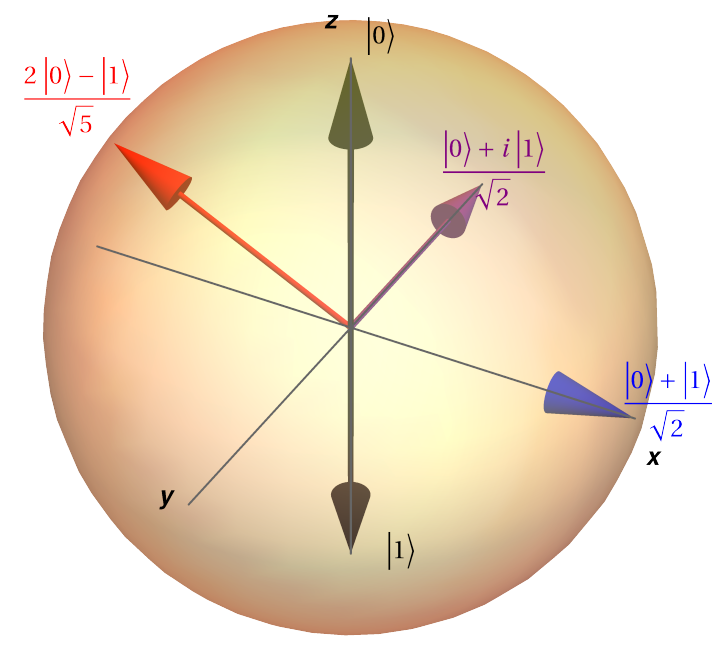
\includegraphics[width=5cm]{bloch.png}
\end{minipage}
$\stackrel{\E_{z}\otimes\1 \vspace{1cm}}{\longmapsto}$
\begin{minipage}{0.4\textwidth}
\centering
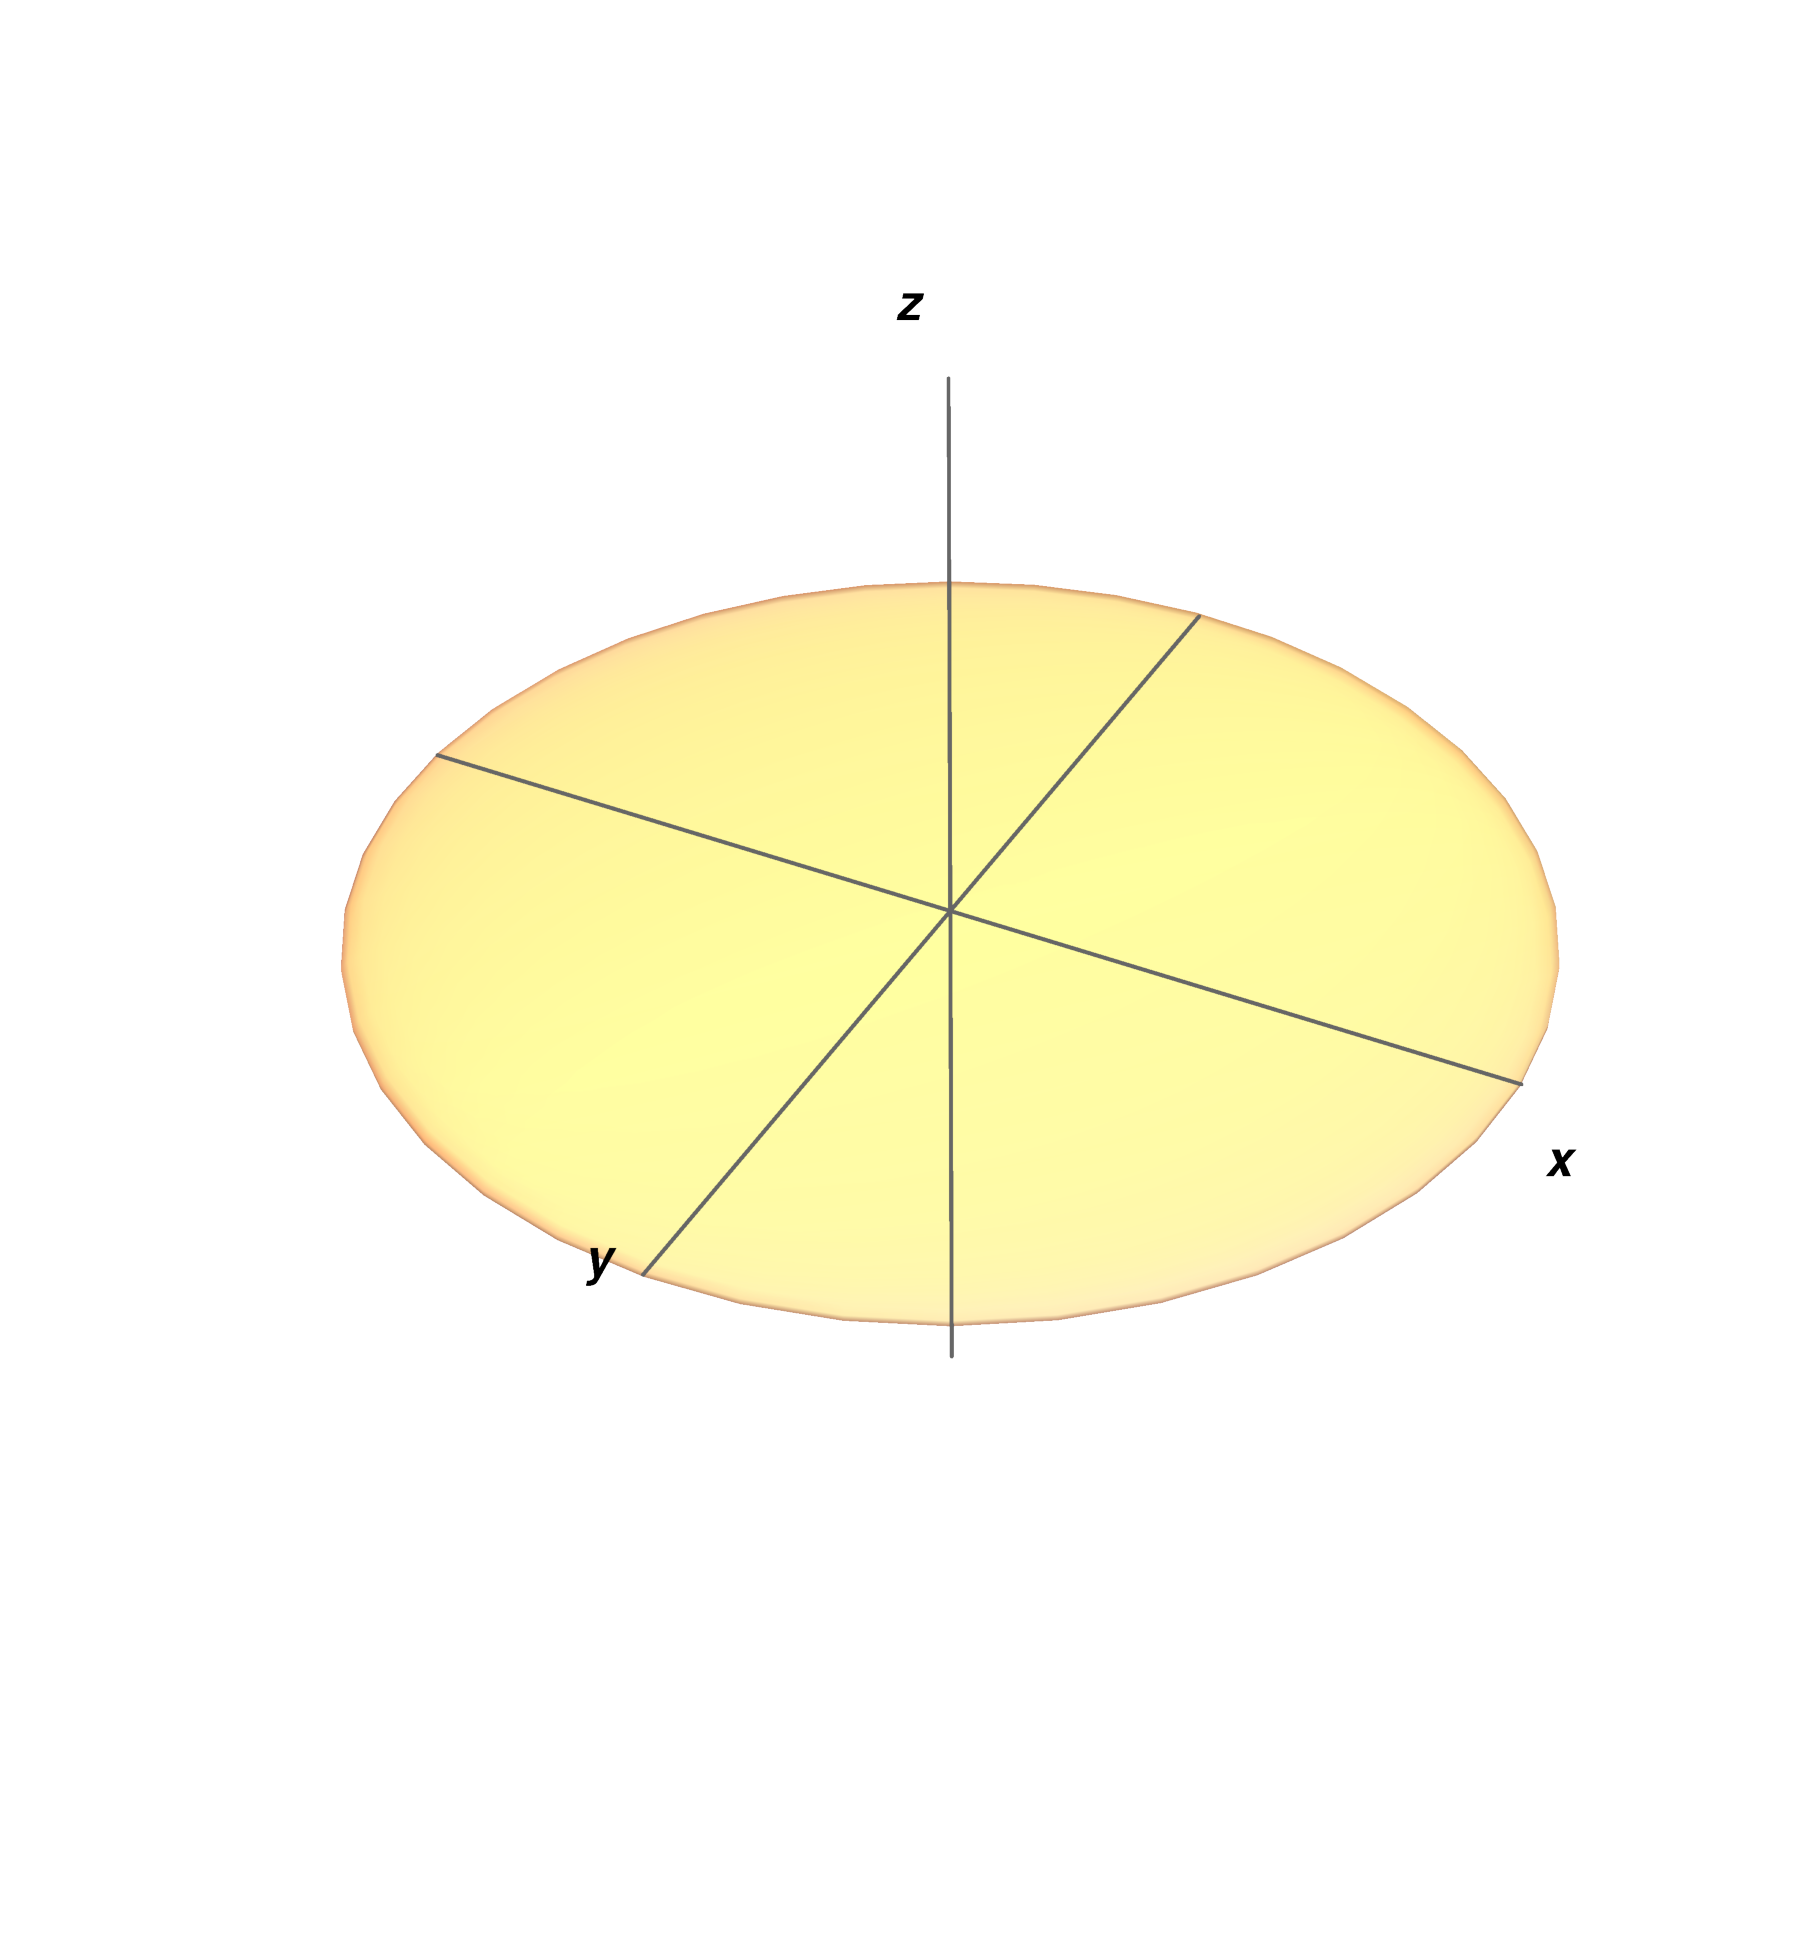
\includegraphics[width=6cm]{DiskXY}
\end{minipage}
\caption{
Deformación de la esfera de Bloch a un disco sobre el plano $XY$.}
\label{fig:qtm-op-motivation}
\end{figure} % }}}

El estado máximamente entrelazado de 2 qubits es
$\ket{\phi}=\qty(\ket{0}+\ket{1})/\sqrt{2}$~\cite{bengtsson_zyczkowski_2017}.
Ya que conocemos cómo transforma $\E_z$ a las componentes de 
la matriz de densidad escrita en la base de Pauli es necesario calcular 
la representación de $\dyad{\phi}{\phi}$ en esa base.
Las componentes $r_{ij}$ se calculan a partir de las
proyecciones de $\dyad{\phi}{\phi}$ sobre los elementos 
$\sigma_i\otimes\sigma_j$ usando el producto interno
de Hilbert-Schmidt $\Tr\qty(\pauli{i}{j}\dyad{\phi}{\phi})$.
Así, se encuentra que
\begin{align}
\dyad{\phi}{\phi}=
\pauli{0}{0}+\pauli{1}{1}-\pauli{2}{2}+\pauli{3}{3}.
\end{align}

Ya que $\E_z$ borra la componente $z$ del vector de Bloch, 
entonces la acción de $\E_z\otimes\1$ debe ser tal que borra 
las componentes de la forma $r_{3j}$ de $\dyad{\phi}{\phi}$, 
por lo cual
\begin{align}
\E_z\otimes\1 \qty({\rho}^{\phi})=
\pauli{0}{0}+\pauli{1}{1}-\pauli{2}{2};
\end{align}
y, transformando de vuelta a la base computacional,
\begin{align}
\E_z\otimes\1 \qty(\dyad{\phi}{\phi})=
\mqty( 
\frac{1}{4} & 0 & 0 & \frac{1}{2} \\
0 & \frac{1}{4} & 0 & 0 \\
0 & 0 & \frac{1}{4} & 0 \\
\frac{1}{2} & 0 & 0 & \frac{1}{4} \\
).
\end{align}
La matriz  $\E_z\otimes\1\qty(\dyad{\phi}{\phi})$ tiene un 
eigenvalor igual a $-1/4$ y, por lo tanto, no es una matriz de densidad.  
Dicho de otro modo, $\E_z\otimes\1\qty(\dyad{\phi}{\phi})$ 
no cumple con una de las condiciones para representar un estado físico
de un sistema de 2 qubits. Hemos mostrado con este ejemplo que la completa 
positividad es una condición más fuerte a la de la positividad para 
asegurar que todos los estados de un sistema, incluyendo a 
cualquier posible estado entrelazado con otro sistema, se transforman
en estados físicos.

Ahora vamos a establecer la condición de completa positividad 
de forma precisa. Se dice que una operación $\E$ es CP si 
y sólo si, para cualquier extensión arbitraria de dimensión $K$ 
del espacio de Hilbert $(\hi_N \rightarrow \hi_N \otimes \hi_K)$ 
el operador $\E\otimes\1_K$ es positivo~\cite{bengtsson_zyczkowski_2017}. 
Con esta condición las restricciones sobre un canal cuántico 
para que este describa una evolución física están completas.

Un canal cuántico es un mapeo lineal que  (1) preserva las características
de las matrices de densidad y (2) es completamente positivo. 
En la literatura se suele utilizar el término operaciones 
completamente positivas que preservan la traza 
(CPTP) para referirse a los canales 
cuánticos~\cite{bengtsson_zyczkowski_2017}. 
Ahora que hemos establecido las condiciones que satisfacen los
canales cuánticos vamos a presentar en la siguiente sección 
dos formas distintas, pero equivalentes, de representar a un canal 
cuántico: como superoperador y la forma de Kraus.


% }}}
\section{Representaciones de los canales cuánticos} % {{{
\label{sec:qtm-channels-representation}
\esqueleto{Enunciar que existen las representaciones de 
Kraus y de superoperador. Copy-paste de las secciones en las 
que hablamos de las representaciones en el informe final. Planeo
dejar sólo un ejemplo y matar los ejemplos de las dos representaciones
en un tiro.}

Los canales cuánticos pueden representarse como superoperadores
o en la representación de suma de operadores de Kraus. 
La matriz de densidad es un operador que actúa sobre el espacio 
de Hilbert, por consiguiente, la ecuación \eqref{eq:E(rho)} 
sugiere que $\E$ es un operador que actúa sobre el espacio 
de Hilbert-Schmidt (espacio en el que viven las matrices de densidad). 
A esta clase de operadores es a los que se les conoce como 
superoperadores~\cite{preskill1998lecture}.
Por otro lado, la representación de Kraus es una forma de 
representar a un canal cuántico con operadores que pertenecen
al mismo espacio en el que se contienen las matrices de densidad.

Un superoperador actúa sobre la matriz de densidad 
como un vector columna. Por ello, discutiremos un procedimiento 
para `vectorizar' a la matriz de densidad.
Consideremos una matriz de densidad $\hat{\rho}$ de dimensión $d\times d$.
La matriz $\hat{\rho}$ puede escribirse como 
un vector columna $\vec{\rho}$, con $d^2$ elementos, 
ordenando los elementos de matriz según la ecuación  
\begin{align}
\rho_k=\hat{\rho}_{ij}, 
\label{eq:matrix-to-vector}
\end{align}
donde $k=\qty(i-1)d+j$, con $i,j=,1,\ldots,d$. 

Para establecer más adelante una manera de evaluar la CP de una operación 
lineal vamos a introducir a continuación una notación de 4 índices para 
etiquetar a los elementos de matriz de un operador que actúa 
sobre un espacio bipartito y una transformación conocida como 
\textit{reshuffle} para reordenar a una matriz. 
Supongamos que $U$ es un operador 
que actúa sobre un espacio de Hilbert 
$\hi$ de la forma $\hi=\hi_M\otimes\hi_N$.
Consideremos una base ortonormal $\ket{m}$ de $\hi_M$ 
y una base ortonormal $\ket{\mu}$ de $\hi_N$. 
Los productos $\ket{m}\otimes\ket{\mu}$ definen a una base
ortonormal del espacio compuesto $\hi$. 
Nótese el uso de letras latinas para los índices del
primer subsistema y letras griegas para los índices del segundo. 
Un elemento de matriz de $U$ se puede etiquetar como
\begin{align}
U_\ind{m\mu}{n\nu}=\matrixel{m\otimes \mu}{U}{n\otimes \nu}.
\label{eq:4indices}
\end{align}
En esta notación de cuatro índices la transformación de \textit{reshuffle}, 
para reordenar a una matriz  $U$, se define 
como~\cite{bengtsson_zyczkowski_2017}
\begin{align}
U^R_\ind{m\mu}{n\nu} = U_\ind{mn}{\mu\nu}.
\label{eq:R-4ind}
\end{align}
Con esta nueva notación y una definición de 
la transformación de \textit{reshuffle}
contamos con las herramientas necesarias para establecer 
las condiciones que un superoperador $\E$ debe satisfacer 
para ser un canal cuántico.

Un canal cuántico es una operación lineal completamente
positiva que preserva las características de la matriz de densidad.
Es decir, un canal cuántico transforma a la matriz de densidad de
tal manera que preserva su (1) Hermiticidad, (2) traza unitaria y 
(3) positividad semidefinida. Para que esto se satisfaga, un 
canal cuántico $\E$ debe cumplir~\cite{bengtsson_zyczkowski_2017}:
\begin{align}
\txt{(i)}&& \rho'=\qty(\rho')^{\dagger}&&\Leftrightarrow
    && \E_\ind{m\mu}{n\nu}=\E_\ind{\mu m}{\nu n}^*,&&
    \label{eq:H-condition}\\
\txt{(ii)}&&\Tr(\rho')=1
    &&\Leftrightarrow&&  \sum_{m}\E_\ind{mm}{n\nu}=\delta_{n\nu},\\     
\txt{(iii)}&&\rho'\geq0
    &&\Leftrightarrow&&  \sum_{n\nu}\E_{\ind{m\mu}{n\nu}}\rho_{n\nu}\geq0 &
    \text{\hspace{8pt}cuando\hspace{4pt}} \rho>0.
    \label{eq:positivity-condition}
\end{align}
Adicionalmente, para evaluar la completa positividad de $\E$ es 
necesario introducir a la matriz de Choi $D_{\E}$ de un canal cuántico.
La matriz $D_{\E}$ se define como la matriz resultante de 
aplicar la transformación de \textit{reshuffle} al superoperador $\E$,
es decir, $D_{\E}=\E^{R}$~\cite{bengtsson_zyczkowski_2017}.
Finalmente, la condición de CP de $\E$, utilizando a su matriz de Choi, 
está establecida en el siguiente teorema.
\begin{thm}{Teorema de Choi.}\label{thm:choi-CP}
Un superoperador lineal $\E$ es completamente positivo si y sólo si 
su matriz de Choi asociada $D_{\E}$ es positiva semidefinida.
\end{thm}
\begin{proof}
Vamos a presentar la demostración expuesta por Bengtsson
en~\cite[p. 281]{bengtsson_zyczkowski_2017}.
La matriz de Choi $D_{\E}$ de un 
canal cuántico $\E$ es una matriz Hermítica que 
actúa sobre el espacio de Hilbert-Schmidt $\mathcal{H}_{N^2}$
(espacio de las matrices de dimensión $N^2\times N^2$). 
Utilizando el teorema de descomposición 
espectral~\cite{nielsen_chuang_2011},
\begin{align}
D_{\E}&=\sum_{i}\lambda_i\dyad{\chi_i}{\chi_i}
&
D_{\ind{mn}{\mu\nu}}&=\sum_i\lambda_i
\chi^i_{mn}\qty(\chi_{\mu\nu}^i)^*,
\end{align}
donde los eigenvalores $\lambda_i\in\mathbb{R}$. Ahora consideremos
la acción de $\E\ot \1_N$ sobre un estado puro $z_{nn'}z^*_{\nu\nu'}$,
\begin{align}
\rho'_{mm'\mu\mu'}&=
\sum_{n,n',\nu,\nu'}
\E_{\ind{m\mu}{n\nu}}\delta_{\ind{m'\mu'}{n'	\nu'}}z_{nn'}z^*_{\nu\nu'}
=
\sum_{n,\nu}
\E_{\ind{m\mu}{n\nu}}z_{nm'}z^*_{\nu\mu'},
\end{align}
donde $\delta_{\ind{m'\mu'}{n'	\nu'}}=\delta_{m'n'}\delta_{\mu'\nu'}$,
\begin{align}
\sum_{n,\nu}\E_{\ind{m\mu}{n\nu}}z_{nm'}z^*_{\nu\mu'}&=
\sum_{n,\nu}D_{\ind{mn}{\mu\nu}}z_{nm'}z^*_{\nu\mu'}\nonumber\\
\rho'_{mm'\mu\mu'}&=
\sum_{n,\nu,i}\lambda_{i}
\chi^i_{mn}z_{nm'}\qty(\chi_{\mu\nu}^iz_{\nu\mu'})^*,
\end{align}
donde utilizamos $\E_{\ind{m\mu}{n\nu}}
=\E^R_{\ind{mn}{\mu\nu}}
=D_{\ind{mn}{\mu\nu}}$.
Finalmente, para evaluar que $\rho'$ sea una matriz de densidad positiva 
calculamos sus elementos de matriz con un vector arbitrario~$y_{mm'}$
para encontrar la condición que se debe de satisfacer,
\begin{align}
\sum_{m,m',\mu,\mu'}
y_{mm'}\rho'_{mm'\mu\mu'}y_{\mu\mu'}=
\sum_{m,m',n,n'}\lambda_i\abs{
y_{mn'}\chi^i_{mn}z_{nm'}}^2
\geq0,
\end{align}
entonces $\lambda_i\geq1$. Por consiguiente, la matriz 
de Choi $D_{\E}$ debe ser positiva semidefinida para que $\rho'$ 
también lo sea.
\end{proof}
En resumen, las condiciones \eqref{eq:H-condition} 
a \eqref{eq:positivity-condition}, más el teorema \eqref{thm:choi-CP},
establecen las restricciones sobre el superoperador $\E$ para que sea
un canal cuántico~\cite{bengtsson_zyczkowski_2017}.

Por el otro lado, un canal cuántico $\E$ también puede escribirse
en la representación de suma de operadores.
En 1971, Karl Kraus introdujo esta representación como resultado
del teorema de Stinespring \cite{bengtsson_zyczkowski_2017}.
La representación de Kraus de un canal cuántico reescribe
a la ecuación \eqref{eq:E(rho)} como
$\E\qty(\rho)=\sum_k E_k\rho E_k^{\dagger}$,
para algún conjunto de operadores $\{E_k\}$ 
que satisfacen la condición 
$\sum _kE_k^{\dagger}E_k\leq\1$~\cite{nielsen_chuang_2011}. 
Esta representación se relaciona con el superoperador $\E$ por
medio de la matriz de Choi.

La representación de Kraus no es única y, por ello, es de interés
determinar un conjunto $\{E_k\}$ de operadores canónicos de $\E$.
Se puede encontrar un conjunto de operadores canónicos de Kraus de 
un canal cuántico $\E$ a partir de los eigenvectores normalizados 
$\ket{\chi_k}$ de la matriz de Choi reordenados como matrices 
mediante el proceso inverso
establecido en \eqref{eq:matrix-to-vector}~\cite{bengtsson_zyczkowski_2017}.
Además, la raíz cuadrada de los eigenvalores $\sqrt{\lambda_k}$ de 
$D_{\E}$ proporcionan los pesos de los operadores canónicos $E_k$.

\textbf{Forma canónica de Kraus.} Un mapeo completamente 
positivo $\E:\mathcal{M}^{(N)}\to\mathcal{M}^{(N)}$ se
puede escribir como
\begin{align}
\rho \longrightarrow \rho' = 
\sum_{k=1}^{r\leq d^2}\lambda_k\chi_k\rho\chi_k^{\dagger}
= \sum_{i=1}^rE_k\rho E_k^{\dagger},
\label{eq:Kraus-canonical}
\end{align}
donde $r$ es el rango de $D_{\E}$ y $\chi_k$ sus eigenvectores
$\ket{\chi_k}$ reordenados como matrices. Esto quiere decir que 
$E_k=\sqrt{\lambda_k}\chi_k$. Además, los 
operadores $E_k$ deben satisfacer la condición
\begin{align}
  \Tr\qty(E_i^{\dagger}E_j)=d_i\delta_{ij}.
  \label{eq:Tr-Kraus-canonical}
\end{align}
Si canal cuántico $\E$ preserva la $\Tr \rho$, se cumple que
\begin{align}
  \sum_kE_k^{\dagger}E_k=\1
  \hspace{0.5cm}\Rightarrow\hspace{0.5cm}
  \sum_{k=1}^r\lambda_k=N .
  \label{eq:completeness-Kraus-canonical}
\end{align}
Se conoce como rango de Kraus al número de operadores 
en la forma canónica. Es decir, el número de términos en la sumatoria
en \eqref{eq:Kraus-canonical}. Por consiguiente, el rango de 
Kraus de $\E$ es igual al rango de su matriz de Choi 
$D_{\E}$~\cite{bengtsson_zyczkowski_2017}.

Con esto completamos los fundamentos teóricos para estudiar 
el problema de las operaciones PCE a partir del siguiente capítulo. 
Primero presentamos a la matriz de densidad como una herramienta 
para representar a los estados cuánticos. Luego, expusimos la teoría 
de los canales cuánticos para estudiar la dinámica de los sistemas 
cuánticos abiertos. Un canal cuántico es una operación
completamente positiva que preserva las características de la 
matriz de densidad. Ahora nos vamos a centrar en estudiar una 
dinámica muy particular de los sistemas de qubits.
% }}}
%%% Lo que está comentado abajo era parte del modelo, puede ser útil  después  {{{
%%%%%%%%%%%%%%%%%%%%%%%%%%%%%%%%%%%%%%

%En adición a los conjuntos de puntos que se trabajan con normalidad
%en Matemáticas ~---puras y aplicadas---, se tendrá que hacer uso
%frecuentemente de los conjuntos de conjuntos, si por ejemplo $X$ es
%la recta real, como un intervalo es un conjunto de puntos, es decir
%un subconjuto de $X$, se tendrá que el conjunto de todos los
%intervalos es un conjunto de conjuntos.
%
%En especial, cuando una clase hace referencia a subconjuntos del
%conjunto $X$, la llamaremos \textbf{familia}. En especial el
%\textbf{conjunto potencia} $\mathcal{P} (X)=\{A\mid A\subseteq X\}$
%es una familia de $X$. Asimismo, se definirá el \textbf{complemento}
%de $A$ por \[A^c=\{x\mid x\notin A\}.\]
%
%\begin{defn}\label{dfcp28} Una \textbf{función de selección}
%para un conjunto $X$ es una función $f$ la cual asocia a cada
%subconjunto no vacío $E$ de $X$ un elemento de $E$: $f(E)\in E$.
%\end{defn}
%
%\begin{axm}[de selección]\label{choice} Para cualquier conjunto
%existe una función de selección.
%\end{axm}
%
%\begin{rem} Con frecuencia el axioma~\ref{choice} se presenta en
%la forma: para cada $E\in \mathcal{P}(X)\setminus\{\nada\}$,
%elegimos un elemento $x\in E$. Asimismo, es equivalente al lema de
%Zorn, para más detalles consultar
%~\cite[p. 97]{Halmo},~\cite[p. 338]{Haus} o~\cite[p. 14]{Hewit}.
%\end{rem}
%
%Una \textbf{clase disjunta} es una clase {\boldmath $A$} de
%conjuntos tal que para cualquier par de conjuntos distintos de
%{\boldmath $A$} son disjuntos, en este caso nos referiremos a la
%unión de conjuntos de {\boldmath $A$} como \textbf{unión disjunta}.
%
%Si $E$ es un subconjunto de $X$, la función $\chi _E$ definida para
%$x\in X$ por la relación:
%\begin{equation}\label{eq0}
%    \chi_E(x)= \begin{cases}
%    1, & \mbox{si } x\in E, \\
%    0, & \mbox{si } x\notin E.
%    \end{cases}
%\end{equation}Es llamada \textbf{función característica}
%del conjunto $E$. La correspondencia entre los conjuntos y sus
%funciones características es inyectiva, y todas las propiedades de
%conjuntos y operaciones entre conjuntos pueden ser expresadas por
%medio de funciones características. 
%
%%%%	TABLA CORTA, ÚNICAMENTE LLEVA LÍNEAS HORIZONTALES PARA SEPARAR BLOQUES
%
%\begin{table}[ht]
%\caption[título optativo de la tabla]{Propiedades de los espacios $L^p$. Fuente: tomada de \cite[Cap. 3]{Brez}.}\label{tablaLp}
%\centering
%\begin{tabular}{cccc}
%\hline
%Espacio & Reflexivo\footnote{En el sentido topológico.} & Separable & Dual \\ \hline %\hline
%$L^p$, $1<p<\infty$  & Si & Si & $L^q$, $1/p+1/q=1$ \\
%$L^1$ & No & Si & $L^\infty$ \\
%$L^\infty$ & No & No & $L^1 \varsubsetneq (L^\infty)’$ \\ \hline
%\end{tabular}
%\end{table}\footnotetext{En el sentido topológico.} 
%
%\begin{defn}\label{dfcp1}Si $\su En$ es una sucesión de
%conjuntos, definiremos los conjuntos $\overline{\lim } E_n$ y
%$\underline{\lim } E_n$ de la siguiente forma:
%\[\begin{array}{cc}
%  \overline{\lim} E_n=\limsup \limits_{n\rightarrow \infty}E_n =
%  \bigcap \limits_{n=1}^\infty \Union Ein \infty ,&
%  \underline{\lim} E_n=\liminf \limits_{n\rightarrow \infty}E_n =
%  \bigcup \limits_{n=1}^\infty \Inter Ein \infty \\
%\end{array}\] y los llamaremos \textbf{límite superior} y
%\textbf{límite inferior}, respectivamente, de la sucesión $\su En$.
%Si tenemos $\overline{\lim} E_n = \underline{\lim} E_n$, usaremos la
%notación $\lim_n E_n$ para este conjunto. Si la sucesión es tal que
%$E_n\subset E_{n+1},\ n=1,2,\dots$ le llamaremos \textbf{creciente}
%y se denotará por $E_n\!\!\uparrow$ y su límite será $\lim
%\limits_{n\rightarrow \infty}E_n = \union En1 \infty$; si es tal que
%$E_n\supset E_{n+1},\ n=1,2,\dots$ le llamaremos
%\textbf{decreciente} y se denotará por $E_n\!\!\downarrow$ y su
%límite será $\lim \limits_ {n\rightarrow \infty}E_n = \inter En1
%\infty$. En ambos casos nos referiremos a ella como
%\textbf{monótona}.\end{defn}
%
%
%\begin{defn}\label{dfcp2}Sea $f$ una aplicación definida del conjunto
%$X$ al conjunto $Y$, es decir $f:X\To Y$. Para cualquier subconjunto
%$T\subseteq Y$, definimos la \textbf{imagen inversa} de $T$, bajo
%$f$, denotada por $\ff (T)$, como sigue:
%\[\ff (T)=\{s\in X\mid f(s)\in T\}.\]\end{defn} 
%
%\begin{thm}\label{thcp1}Para la aplicación $\ff :{\cal{P}} (Y)
%\To {\cal{P}} (X)$ se tienen las propiedades siguientes:
%\begin{enumerate}
%    \vspace{0pt} \item $\ff(\bigcup_j T_j) = \bigcup_j
%    \ff(T_j)$.
%    \vspace{0pt} \item $\ff(\bigcap_j T_j) = \bigcap_j
%    \ff(T_j)$.
%    \vspace{-6pt} \item Si $T_1\cap T_2=\nada$, entonces
%    $\ff(T_1)\cap \ff(T_2) = \nada$.
%    \vspace{-6pt} \item $\ff(T^c) = [\ff(T)]^c$.
%    \vspace{-6pt} \item $\ff(\nada) = \nada$.
%    \vspace{-6pt} \item $\ff(Y) = X$.
%\end{enumerate}
%\end{thm}
%
%
%Las propiedades (1) y (3) del teorema~\ref{thcp1} establecen las
%condiciones para la unión disjunta en una familia en $Y$. Sea ahora
%$\Df$ una familia cualquiera de subconjuntos de $Y$, y definamos la
%familia $\ff (\Df)$ de subconjuntos de $X$ como
%sigue:\begin{equation}\label{eq1}
%    \ff(\Df) = \{A\subseteq X \mid
%A = \ff(T) \mbox{ para algún } T\in \Df\} = \{\ff(T) \mid T\in
%\Df\}.
%\end{equation}
%
%El sistema de numeros reales extendido o \textbf{recta real
%extendida} es el conjunto definido por $\RR\df\R \cup \{-\infty,
%+\infty\}$, con la siguiente relación de orden: para $a\in \R$
%tenemos $-\infty <a< +\infty$. La topología para este conjunto se
%define por declarar como abiertos a los siguientes conjuntos:
%$(a,b),\ [-\infty,b),\ (a,+\infty]$ y cualquier unión de conjuntos
%de este tipo. Cuando se haga referencia a los \textbf{numeros reales
%extendidos} o \textbf{valor real extendido}, se estará hablando de
%los numeros reales y de los símbolos $\pm\infty$. Cuando trabajamos
%con teoría de la integración, nos encontraremos con $\infty$, una
%razón es que algunas veces trataremos de integrar sobre conjuntos de
%medida infinita, este es caso de la recta real.
%
%Por tal motivo, se hacen las siguientes definiciones para
%facilitar su manejo: $a+\infty = \infty+a \df \infty$ si $0\leq a
%\leq \infty$,~y
%\begin{equation}\label{eq4}
%    a\cdot \infty = \infty \cdot a
%\df\begin{cases}
%  \infty, & \mbox{si } 0 < a \leq \infty \\
%  0, & \mbox{si } a = 0 \\
%\end{cases}
%\end{equation}las leyes de cancelación se tratan
%así: $a+b = a+c\ \Rightarrow\ b=c\ $ y $a\cdot b =a\cdot c\
%\Rightarrow\ b=c$ sólo cuando $0 < a < \infty$. 
%
%\begin{defn}\label{dfcp3}Sea $\su aj$ una sucesión en la recta
%real extendida, y sean $b_k = \sup\{a_k,a_{k+1},a_{k+2}\dots\},\
%k=1,2,3,\dots$, y $\beta = \inf\{b_1,b_2,b_3,\dots\}$. Entonces
%llamaremos a $\beta$ el \textbf{límite superior} de $\su aj$, y
%escribiremos $\beta = \limsup \limits_{j\rightarrow \infty}(a_j)$.
%El \textbf{límite inferior} se define análogamente, al intercambiar
%$\sup$ e $\inf$ en las anteriores definiciones; notemos que \[\liminf
%\limits_{j\rightarrow \infty}(a_j) = -\limsup \limits_{j\rightarrow
%\infty}(-a_j).\] Si $\su aj$ converge, entonces tenemos $\liminf
%\limits_{j\rightarrow \infty}(a_j) = \limsup \limits_{j\rightarrow
%\infty}(a_j) = \lim \limits_{j\rightarrow
%\infty}(a_j)$.\end{defn}
%
%\begin{prp}\label{prcp1}Si $0\leq a_1\leq a_2\leq \cdots$,
%$0\leq b_1\leq b_2\leq \cdots$, tales que $a_j \To a$ y $b_j \To
%b$. Entonces $a_j b_j \To ab$.
%\end{prp}
%
%\begin{defn}\label{dfcp4}Supongamos que $\su fj$ es una sucesión de
%funciones de valor real extendido en un conjunto $X$. Entonces
%$\sup_j f_j$ y $\limsup \limits_{j\rightarrow \infty} f_j$ son las
%funciones definidas en $X$ por:
%\[\left(\sup_j f_j\right)(x)\df \sup_j(f_j(x)),\quad \left(\limsup
%\limits_{j \rightarrow \infty} f_j\right)(x)\df \limsup \limits_{j
%\rightarrow \infty}(f_j(x)).\] Si $f(x)=\lim \limits_{j \rightarrow
%\infty} f_j(x)$, y asumimos que el límite existe para cualquier
%$x\in X$, entonces llamaremos a $f$ el \textbf{límite puntual} de la
%sucesión $\su fj$ y hablaremos de \textbf{convergencia puntual} en
%este contexto.\end{defn}
%
%\begin{figure}[ht]
%\centering
%\label{fig:analisisGraficoModelo3}
%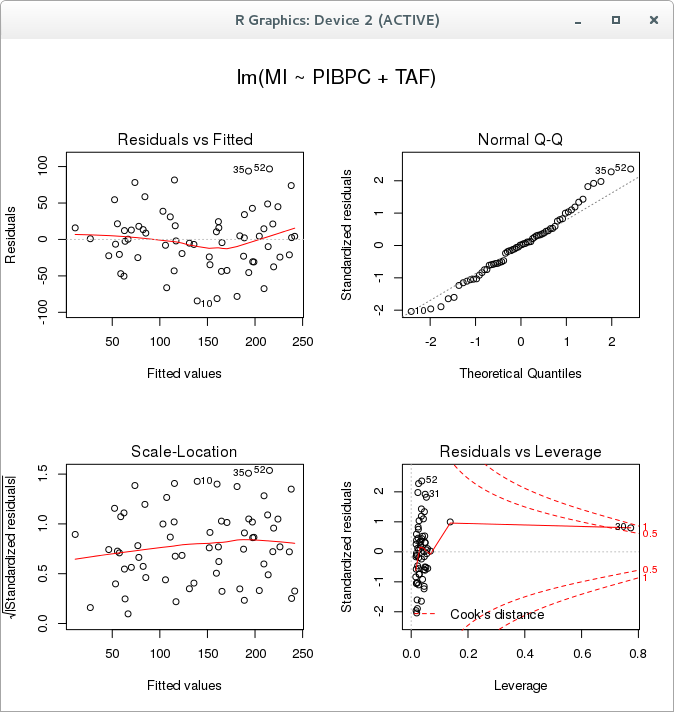
\includegraphics[width=0.9\linewidth]{analisisGraficoModelo3}\\
%\caption[Titulo en el índice de figuras (opcional)]{Título en el 
%documento. Las imágenes pueden ser raster (de preferencia jpg, png 
%con buena resolución para imprimir) o vectorial (convertir a pdf, en 
%este caso la resolución no afecta) Fuente: imagen tomada de~\cite{liu}.}
%\end{figure}
%
%
%\begin{lem}\label{lmcp11}Sean $z,w \in \C$, $1 < p \leq 2$ y $1/p +
%1/q = 1$. Entonces tenemos \[\abs{z+w}^q + \abs{z-w}^q \leq 2 (|z|^p
%+ |w|^p)^{\frac{1}{p-1}}.\]
%\end{lem}
%
%\begin{proof} Consultar~\cite[p. 227]{Hewit}. \end{proof}
%
%\begin{defn}\label{dfcp5}Sea $f:X\To \RR$ una aplicación. Se definen
%las aplicaciones $f^+\!\df\max\{f,0\}$, $f^-\!\df-\min\{f,0\}$, a
%$f^+$ y $f^-$ se les llama la \textbf{parte positiva y negativa} de
%$f$, respectivamente.
%\end{defn}
%
%
%\begin{prp}\label{prcp2}Para cualquier aplicación $f:X\To \R$
%denotaremos su valor absoluto con $\abs f$, entonces tenemos
%\[\abs f=f^++f^-,\quad f=f^+-f^-.\]
%\end{prp}
%
%% --------------->  
%
%\section{Tablas y Gráficas}
%
%Las tablas y gráficas deben tener un título \verb|\caption{text}| que la identifique, debe especificar la \textbf{fuente}, y una etiqueta \verb|\label{text}| para hacer referencias cruzadas dentro del documento.
%
%%% TABLAS LARGAS LLEVAN TODAS LAS DIVISIONES DE LOS BLOQUES
%\subsection{Tablas}
%
%\begin{longtable}{|l|l|l|l|l|}
%\caption[]{Diccionario de datos, tabla \textit{marn} (continuación)} \\ \hline
%
%\multicolumn{1}{|c|}{\textbf{Name}} & \multicolumn{1}{c|}{\textbf{Data type}} & \multicolumn{1}{c|}{\textbf{Not Null?}} & \multicolumn{1}{c|}{\textbf{Primary key?}} & \multicolumn{1}{c|}{\textbf{Default}} \\ \hline \endhead
%	\caption[Diccionario de datos, tabla \textit{marn}]{Diccionario de datos, tabla \textit{marn}. Fuente: obtenida de pgAdminIII}\label{data:marn} \\ \hline
%
%	\multicolumn{1}{|c|}{\textbf{Name}} & \multicolumn{1}{c|}{\textbf{Data type}} & \multicolumn{1}{c|}{\textbf{Not Null?}} & \multicolumn{1}{c|}{\textbf{Primary key?}} & \multicolumn{1}{c|}{\textbf{Default}} \\ \hline \endfirsthead 
%
%	id & \textit{integer} & \textit{Yes} & \textit{Yes} & \textit{nextval('marn\_id\_seq'} \\ %\hline
%
%	 &  &  &  & \textit{::regclass)}\footnote{Note que la tabla es mas ancha que lo preestablecido. Procure diseñar elementos acordes con el espacio preestablecido.} \\ \hline
%
%	\multicolumn{ 5}{|l|}{Clave primaria que  obtendrá su valor de forma secuencial al ingresar un nuevo registro} \\ \hline
%		lista\_tax & \textit{text} & \textit{No} & \textit{No} & \textit{} \\ \hline
%
%	\multicolumn{ 5}{|l|}{Clasificación del proyecto en base al Listado Taxativo del MARN} \\ \hline
%		no\_marn & \textit{text} & \textit{No} & \textit{No} & \textit{} \\ \hline
%
%	\multicolumn{ 5}{|l|}{Numero de expediente asignado por el MARN} \\ \hline
%		date0 & \textit{date} & \textit{No} & \textit{No} & \textit{} \\ \hline
%
%	\multicolumn{ 5}{|l|}{Día del ingreso del expediente del proyecto (instrumento ambiental) en el MARN} \\ \hline
%		notas & \textit{text} & \textit{No} & \textit{No} & \textit{} \\ \hline
%
%	\multicolumn{ 5}{|l|}{Observaciones} \\ \hline
%		no\_res\_ap & \textit{text} & \textit{No} & \textit{No} & \textit{} \\ \hline
%
%	\multicolumn{ 5}{|l|}{Numero de resolución aprobatoria del proyecto por el MARN%
%	\footnote{Note que en esta línea la tabla se corta y continua en la siguiente página. 
%	Utilizar paquete \textsf{longtable} y ambiente \textit{longtable}.}} \\ \hline
%		date\_res\_ap & \textit{date} & \textit{No} & \textit{No} & \textit{} \\ \hline
%
%	\multicolumn{ 5}{|l|}{Día de emisión de la resolución aprobatoria por el MARN} \\ \hline
%		date0\_fianza & \textit{date} & \textit{No} & \textit{No} & \textit{} \\ \hline
%
%	\multicolumn{ 5}{|l|}{Día de emisión de fianza del proyecto.} \\ \hline
%		no\_res\_fianza & \textit{text} & \textit{No} & \textit{No} & \textit{} \\ \hline
%
%	\multicolumn{ 5}{|l|}{Numero de la resolución de aceptación de fianza por el MARN} \\ \hline
%		date1\_fianza & \textit{date} & \textit{No} & \textit{No} & \textit{} \\ \hline
%
%	\multicolumn{ 5}{|l|}{Fecha de inicio de fianza} \\ \hline
%		date2\_fianza & \textit{date} & \textit{No} & \textit{No} & \textit{} \\ \hline
%
%	\multicolumn{ 5}{|l|}{Fecha de finalización de fianza (renovación)} \\ \hline
%		lic\_ambiental & \textit{text} & \textit{No} & \textit{No} & \textit{} \\ \hline
%
%	\multicolumn{ 5}{|l|}{Numero de licencia ambiental} \\ \hline
%		date\_lic\_ambiental & \textit{date} & \textit{No} & \textit{No} & \textit{} \\ \hline
%
%	\multicolumn{ 5}{|l|}{Fecha de finalización de ultima licencia ambiental} \\ \hline
%		proyecto\_id & \textit{integer} & \textit{Yes} & \textit{No} & \textit{} \\ \hline
%
%	\multicolumn{ 5}{|l|}{Enlace con la tabla proyecto\_id} \\ \hline
%\end{longtable}

% }}}


      % Cap. 1 

\chapter{OPERACIONES PCE}

\section{Introducción} % {{{
\janote{La intro recién la escribí. No la has leído aún, Carlos.}

Este capítulo es el corazón de este manuscrito de tesis. En este capítulo discutimos 
una motivación para definir y estudiar las operaciones PCE de $n$ qubits en la 
sección \ref{sec:PCE_operations}. Partimos de discutir algunos canales cuánticos 
de 1 qubit como \textit{bit-flip} y \textit{defasing} 
\cite{bengtsson_zyczkowski_2017,nielsen_chuang_2011},
específicamente centramos nuestra atención en unos casos particulares
de estos canales para motivar la generalización
de este tipo de operaciones para sistemas de $n$ qubits que bautizamos 
con el nombre de \textit{Pauli component erasing} (PCE). 
Luego, en la sección \ref{sec:1_qubit_problem} resolvemos analíticamente 
el problema de encontrar los canales cuánticos PCE de 1 qubit, 
y en la sección \ref{sec:n_qubits_problem} discutimos 
el algoritmo para resolver el problema de $n$ qubits y la dificultad analítica, 
en contraste con el problema de 1 qubit, que hace que el problema sea 
difícil de resolver de manera exacta. Finalmente, en la sección 
\ref{sec:ch2_solucionNumerica} presentamos las herramientas computacionales 
para implementar un método numérico para encontrar los canales cuánticos 
PCE de 2 qubits y parcialmente los de 3 qubits. 

% }}}
\section{Operaciones PCE} % {{{ 
\label{sec:PCE_operations}
%\esqueleto{
%Dos o tres párrafos máximo hablando sobre las operaciones PCE 
%como operaciones proyectivas a la base de productos tensoriales de 
%las matrices de Pauli. Me gustaría poner un problema de motivación
%sólo para hacer más interesante la lectura a partir de acá y dejarle al
%lector algo con lo que pueda entender qué onda con las operaciones 
%PCE. Propongo lo siguiente: cadena de espines. Supongamos una 
%cadena de espines de $N$ sitios y decimos que nos interesa saber 
%si la matriz de densidad del $i$-ésimo espín puede proyectarse 
%al subespacio cuya base son $\sigma_x$ y $\sigma_y$ (lo que 
%quiero decir es que $(r_x,r_y,r_z)\to(r_x,r_y,0)$). Entonces hablo 
%de que hay que considerar que el $i$-ésimo espín puede estar 
%entrelazado con el resto de la cadena, sin embargo, basta con considerar
%que se encuentra entrelazado con cualquiera de sus vecinos y revisar 
%en qué se transforma la matriz de densidad de esos dos espines para 
%averiguar si es posible tal evolución física. Me gustaría poner unas 
%figuritas para hacer interesante esto. 
%}

%\esqueleto{La idea central de esta sección será: No todas las operaciones que 
%borran componentes de Pauli de la matriz de densidad de 1 qubit no 
%son canales cuánticos.}
%
%\esqueleto{Introducir los canales cuánticos de 1 qubit 
%de bit-flip y defasing como una motivación para definir qué es una 
%operación PCE. Figuritas para la interpretación geométrica y discutir 
%especialmente cómo actúan sobre las componentes de Pauli.}

En esta sección vamos a elaborar una discusión que conducirá a
la definición de una operación PCE y al planteamiento del problema
a tratar en esta tesis. 
Comenzaremos por introducir a los canales cuánticos  
\textit{bit-flip} y \textit{defasing} de 1 qubit. 
Ambos canales cuánticos son operaciones que mapean 
la esfera de Bloch a un elipsoide con eje mayor sobre los ejes $x$ y $z$, 
como se muestra en las Figs. \ref{fig:bit-flip} y \ref{fig:phase-flip}, 
respectivamente.
\begin{figure}
\centering
\begin{minipage}{.4\textwidth}
    \centering
    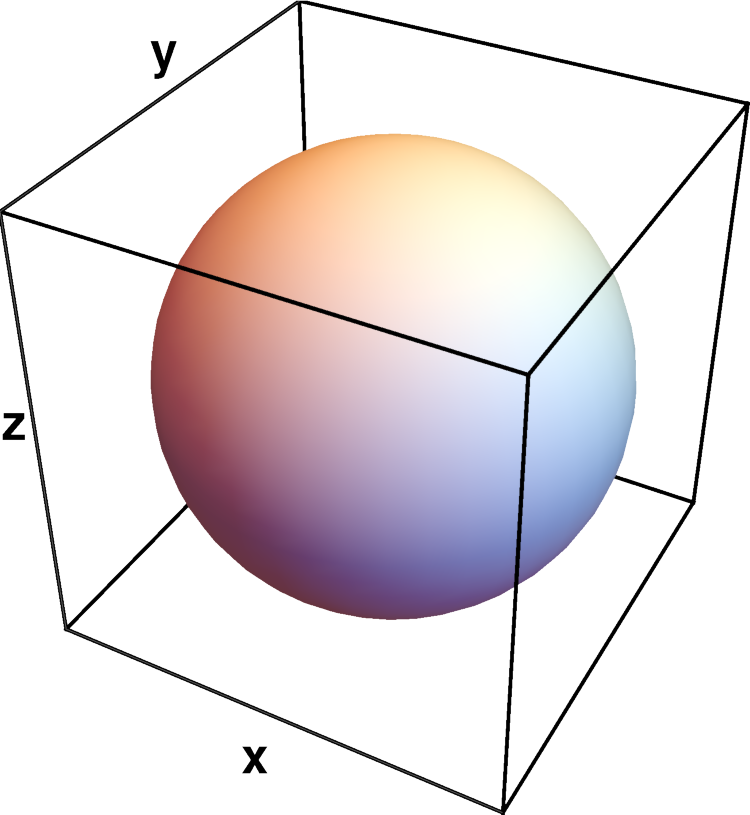
\includegraphics[width=3.8cm]{bloch-ball}
\end{minipage}
\LARGE{$\longmapsto$}
\begin{minipage}{0.4\textwidth}
    \centering
    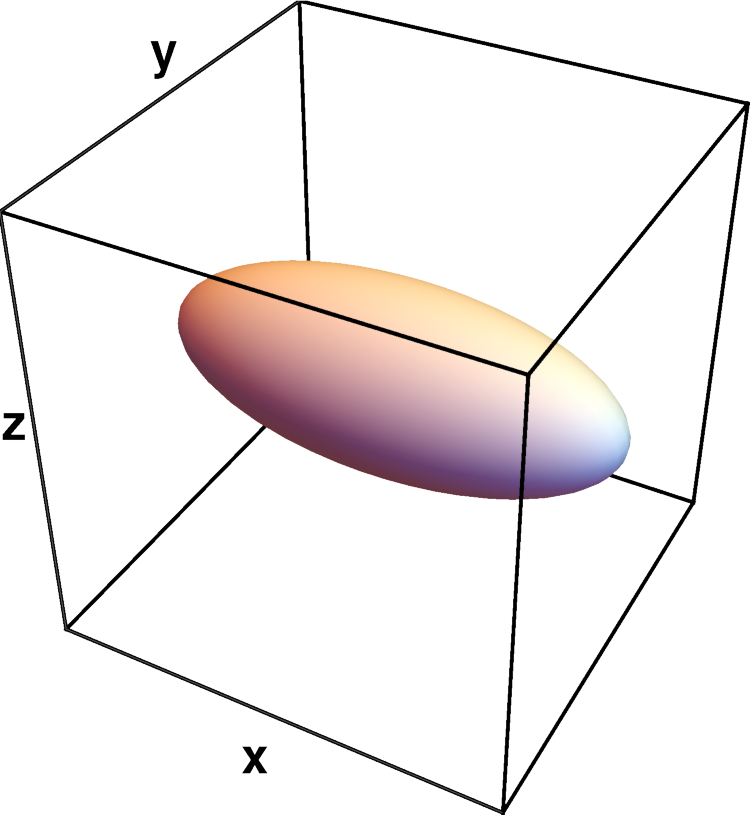
\includegraphics[width=3.8cm]{bit-flip}
\end{minipage}
\caption{
Efecto del canal de inversión de bit sobre la esfera de Bloch, para $p=0.3$. \ep}
\label{fig:bit-flip}
\end{figure}
Para entender algebraicamente cómo actúan estos canales cuánticos 
recordemos que la matriz de densidad de 1 qubit se escribe en la 
base de matrices de Pauli como
\begin{align}\label{eq:rho-1qubit-ch2}
\rho=\frac{1}{2}\sum_{i=0}^3r_i\sigma_i,\hspace{2cm}r_0=1,
\end{align}
donde $r_1$, $r_2$ y $r_3$ especifican las coordenadas $\qty(x,y,z)$ 
del vector de Bloch. El canal \textit{bit-flip} transforma a las componentes 
de \eqref{eq:rho-1qubit-ch2} como~\cite{nielsen_chuang_2011}
\begin{align}\label{eq:bit-flip-transformation}
\qty(1,r_1,r_2,r_3)\longmapsto \qty(1,r_1,(1-2p)r_2,(1-2p)r_3),
\hspace{.5cm} 0\leq p\leq 1.
\end{align}
% \cpnote{Para $p=-1$ si es un canal cuantico? no, hay algo acá que está mal.}
% \janote{Me confundí, pero corregido}
Similarmente, el canal \textit{defasing} actúa sobre las mismas
componentes $r_i$ de \eqref{eq:rho-1qubit-ch2}
como~\cite{nielsen_chuang_2011}
\begin{align}\label{eq:defasing-transformation}
\qty(1,r_1,r_2,r_3)\longmapsto \qty(1,(1-2p)r_1,(1-2p)r_2,r_3),
\hspace{.5cm} 0\leq p\leq 1.
\end{align}
\begin{figure}
\centering
\begin{minipage}{.4\textwidth}
    \centering
    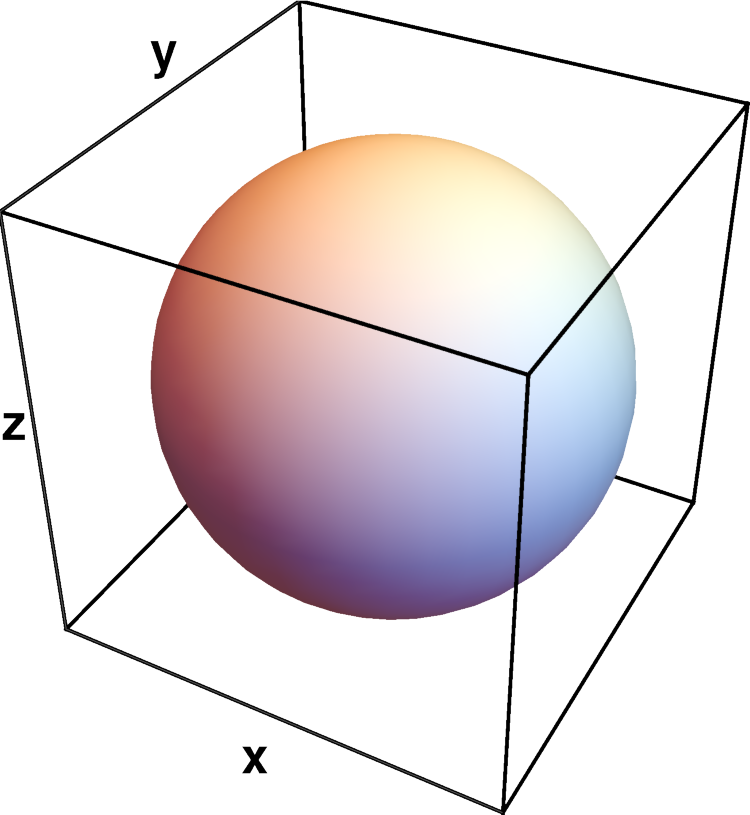
\includegraphics[width=4cm]{bloch-ball}
\end{minipage}
\LARGE{$\longmapsto$}
\begin{minipage}{0.4\textwidth}
    \centering
    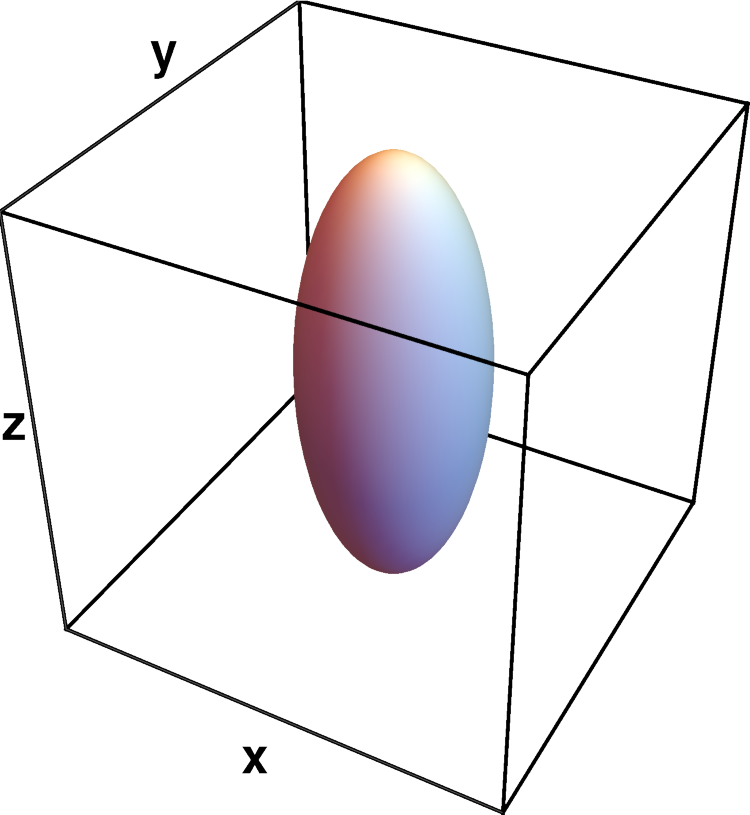
\includegraphics[width=4cm]{phase-flip}
\end{minipage}
\caption{
Acción geométrica del canal defasing de 1 qubit sobre la 
esfera de Bloch, para $p=0.3$. \ep}
\label{fig:phase-flip}
\end{figure}
%\esqueleto{Mencionar los casos del bit-flip y defasing
%cuando la esfera de Bloch se mapea a una linea sobre los ejes $x$ y $y$,
%respectivamente. Nada nuevo, evidentemente son canales porque son 
%casos particulares de otros que son canales. Introducir el punto de vista
%de esos canales como operaciones que borran componentes.}
Vamos a detenernos a analizar qué ocurre cuando $p=1/2$. 
En este caso, \eqref{eq:bit-flip-transformation} y
\eqref{eq:defasing-transformation} se escriben
\begin{align}\label{eq:bit-flip_p=0.5}
\qty(1,r_1,r_2,r_3)&\longmapsto \qty(1,r_1,0,0),\\
\qty(1,r_1,r_2,r_3)&\longmapsto \qty(1,0,0,r_3).\label{eq:defasing_p=0.5}
\end{align}
Es decir que, el \textit{bit-flip} y \textit{defasing} cuando $p=1/2$
son operaciones que mapean la esfera de Bloch a una línea sobre 
el eje mayor de los elipsoides en las Figs. \ref{fig:bit-flip} y \ref{fig:phase-flip}.
Va a ser útil que interpretemos a estos canales cuánticos 
como operaciones que `borran' dos de las proyecciones
$r_i$  de la matriz de densidad de 1 qubit sobre
las matrices de Pauli y que dejan al resto de componentes $r_j$ invariantes.
% \cpnote{La redacción está como 
% chistosa. Por cierto lo de arrancar diciendo ``probara ser \ldots'' suena a 
% anglisismo. Porfa considera cambiar eso. } 
% \janote{Listo}

%\esqueleto{Conducir al lector a preguntarse: `bueno, entonces deplano
%que puedo borrar cualquier cantidad de componentes de Pauli, ¿no? ¡¿NO?!', 
%pero nel. Recordar que vimos en el capítulo anterior la operación que 
%mapea la esfera de Bloch a un disco sobre el plano $x$-$y$ y no es 
%un canal cuántico... porque no es CP. Es decir, la condición de completa 
%positividad es la que impide que las operaciones que borran componentes 
%de Pauli de 1 qubit sean trivialmente canales cuánticos. Siempre será bueno
%que dedique al menos una frase a recordar la implicación física de la CP: 
%existe por lo menos un estado entrelazado en el espacio de 2 qubits 
%que se mapea a un no estado.}

Las operaciones 	que se describen en \eqref{eq:bit-flip_p=0.5}
y \eqref{eq:defasing_p=0.5} sugieren preguntarse si todas las
operaciones que borran cualesquiera de las componentes $r_i$ 
de la matriz de densidad de 1 qubit 
en \eqref{eq:rho-1qubit-ch2} son canales cuánticos.
La pregunta es relevante porque la respuesta es
que no\cpnote{Se me hace una justificación mala. Quiza podemos quitar
esa frase}\janote{Aquí quiero debatirte porque creo que redactado 
de otra manera puedo convencerte (y porque así es cómo defendería
la motivación del problema en la defensa de tesis). Preguntarnos si 
las operaciones PCE de 1 qubit son trivialmente canales cuánticos y darnos cuenta
que no, porque la CP no es trivialmente satisfecha, me 
parece una motivación fuerte para proponer investigar operaciones 
PCE de más qubits y buscar caracterizar a los canales cuánticos PCE.
Supongamos por un momento que todas las operaciones PCE de 
1 qubit son CP, intuitivamente entonces no habría razón para pensar que la 
CP no es trivialmente satisfecha para los PCE de 2 qubits.
En conclusión, que hayan operaciones PCE de 1 qubit no CP puede ser 
un primer motivo para estudiar 2 qubits.}. En el capítulo anterior, en la sección 
\ref{sec:qtm-channels}, elaboramos el ejemplo de la operación $\E_z$
que borra la componente $r_3$ y demostramos que no es un canal 
cuántico porque no es una operación completamente positiva. 
Vimos que no satisfacer esta condición implica que la operación 
$\E_z\ot\1$, que actúa sobre una matriz de densidad de 2 qubits,
no transforma a la matriz 
de densidad del estado máximamente entrelazado en otra 
matriz de densidad.
Es decir, la operación $\E_z$ es un ejemplo de una 
operación de 1 qubit que borra un subconjunto de las componentes $r_i$ de 
la matriz de densidad \eqref{eq:rho-1qubit-ch2} y que no es canal cuántico.

%\esqueleto{Motivar a pensar que si la CP ya impide que algunas 
%operaciones que borran componentes de Pauli de 1 qubit no sean
%canales cuánticos entonces ¿qué ocurrirá en sistemas de más qubits 
%que ya aparecen correlaciones cuánticas? (porque en el caso de 1 qubit 
%la regla de $2^k$ es necesaria y suficiente, para más qubits también 
%va a importar cuáles componentes se borran y en este punto debería 
%ser una pregunta importante para quien no sepa la respuesta)}

La restricción que impone la completa positividad a un canal cuántico 
vuelve interesante estudiar a los canales cuánticos que borran las componentes 
de la matriz de densidad de un sistema de qubits en la base de matrices 
de Pauli. Revisemos el problema de 2 qubits. La matriz de densidad
se escribe
\begin{align}\label{eq:rho_2qubits_cap2}
\rho = \frac{1}{4}\sum_{i,j=0}^3r_{ij}\sigma_i\ot\sigma_j, 
\hspace{2cm} r_{0,0}=1.
\end{align}
Hay 15 componentes $r_{ij}$ que se podrían borrar o dejar invariantes. 
Por consiguiente, hay $32,768$ $(2^{15})$ operaciones distintas que borran las 
componentes de la matriz de densidad \eqref{eq:rho_2qubits_cap2} de 2 qubits. 
El número de operaciones de este tipo crece de manera doblemente 
\cpnote{de hecho doblemente exponencial} \janote{es cierto}
exponencial 
como $2^{4^n-1}$, con $n$ el número de qubits. Sin embargo, no es 
sólo el crecimiento exponencial en el número de operaciones de este tipo
lo que hace interesante al problema, sino también el hecho de que en 
sistemas de más de 1 qubit aparecen correlaciones cuánticas entre 
las particiones del sistema. Por consiguiente, no es trivial inferir cuáles son los 
canales cuánticos que borran las componentes $r_{ij}$ de 
\eqref{eq:rho_2qubits_cap2} a partir de los canales cuánticos 
de 1 qubit que borran las componentes $r_i$ de \eqref{eq:rho-1qubit-ch2}.

%\esqueleto{Ya, no más rodeos y finiquitar con la expresión de $\rho$ para 
%$n$ qubits en la base de Pauli y definir formalmente una operación PCE.}

Sin más, introducimos ahora la definición de una operación PCE de 
$n$ qubits. La matriz de densidad de un sistema de $n$ qubits, en la base de
productos tensoriales de las matrices de Pauli, se escribe como
\begin{align}\label{eq:rho_n_qubits}
\rho=\frac{1}{2^n}\sum_{j_1,\ldots,j_n=0}^3
r_{j_1,\ldots,j_n}\sigma_{j_1}\ot\ldots\ot\sigma_{j_n},
\hspace{2cm} r_{0,\ldots,0}=1.
\end{align}
Vamos a llamar ``componentes de Pauli'' a los coeficientes $r_{j_1,\ldots,j_n}$
de \eqref{eq:rho_n_qubits}. Las componentes de Pauli son las proyecciones
de la matriz de densidad de un sistema de $n$ qubits sobre los elementos
de la base de productos tensoriales de las matrices de Pauli.
Llamamos una operación que borra las componentes de Pauli, 
operación PCE por sus siglas en inglés (\textit{Pauli
component erasing}), a una operación lineal que actúa sobre una 
matriz de densidad de la forma \eqref{eq:rho_n_qubits} y 
que transforma a las componentes de Pauli como
\begin{align}\label{eq:PCE_definition}
r_{j_1,\ldots,r_n}\longmapsto \tau_{j_1,\ldots,r_n}r_{j_1,\ldots,r_n},
\hspace{1cm} \tau_{j_1,\ldots,r_n} = 0,1,
\hspace{1cm} \tau_{0,\ldots,0}=1.
\end{align}
En otras palabras, una operación PCE es una operación lineal que actúa sobre la
matriz de densidad de $n$ qubits y que borra a algunas de las componentes de
Pauli y deja invariantes al resto.
A las operaciones PCE que satisfacen 
la condición de completa positividad y son, por ende, canales cuánticos,
les llamaremos ``canales cuánticos PCE'' o sólamente ``canales PCE''.

De manera muy puntual, podemos formular el problema para 
este trabajo con la siguiente pregunta: ¿qué características tienen 
en común y qué condiciones satisfacen todos los canales PCE 
de sistemas de 2 y 3 qubits? Dicho de otro modo, 
nuestro objetivo es investigar qué hace de diferente la condición de 
completa positividad a los canales PCE del conjunto de todas las 
operaciones PCE de 2 y 3 qubits.
En las siguientes secciones presentaremos el estudio analítico del 
caso de 1 qubit y el método numérico que diseñamos 
para estudiar sistemas de 2 y 3 qubits. 


% }}}
\section{1 qubit} % {{{
\label{sec:1_qubit_problem}
%\esqueleto{
%Idea central de esta sección: encontrar todos los canales cuánticos PCE 
%de 1 qubit.}
%
%\esqueleto{
%Para resolver el problema lo que haremos será encontrar los eigenvalores 
%de la matriz de Choi del superoperador y así encontrar las condiciones 
%que debe satisfacer una operación PCE de 1 qubit para ser un canal cuántico
%en términos de las $\tau_i$. 
%Escribir al superoperador, en su forma diagonal con las $\tau_i$, 
%que actúa sobre la matriz de densidad de 1 qubit escrita en la base de Pauli. 
%}

El problema de los canales PCE de 1 qubit puede ser resuelto analíticamente
y vamos a discutir cómo en esta sección. 
Vamos a presentar nuestro procedimiento para evaluar analíticamente 
la completa positividad de las operaciones PCE de 1 qubit.
De acuerdo con el teorema \ref{thm:choi-CP}, podemos determinar si
una operación es completamente positiva evaluando que su 
matriz de Choi sea una matriz positiva semidefinida.
Por lo tanto, vamos a buscar diagonalizar la matriz de Choi en 
función de los elementos $\tau_i$ de la operación PCE. Así, evaluar
que todos los eigenvalores sean no negativos para 
cada uno de los arreglos de 1's y 0's de las $\tau_i$ que 
caracteriza a las operaciones PCE de 1 qubit 

Enunciamos ahora nuestro algoritmo para evaluar la completa 
positividad de una operación PCE de 1 qubit. 
\begin{enumerate}
	\item Escribir al superoperador de una operación PCE en 
	la base de matrices de Pauli $\sigma_i$ (con $\sigma_0=\1$), 
	base en la cual es diagonal. En general, en la base de Pauli
	el superoperador de una 	operación PCE de 1 qubit se escribe
	\begin{align} \label{eq:supOp_PCE_1q}
		\Phi=\mqty(\dmat[0]{1,\tau_1,\tau_2,\tau_3}).
	\end{align}
	\item Hacer un cambio de base al superoperador \eqref{eq:supOp_PCE_1q}, 
	de la base de matrices de Pauli a la base computacional, vía $P \Phi P^{-1}$, 
	con
	\begin{align}
		P = \mqty(1&0&0&1\\ 0&1&-i&0\\ 0&1&i&0 \\ 1&0&0&-1).
		%	\mqty(\dmat[0]{1,\tau_1,\tau_2,\tau_3})
		%	\mqty(
		% 	\frac{1}{2} & 0 & 0 & \frac{1}{2} \\
		% 	0 & \frac{1}{2} & \frac{1}{2} & 0 \\
		% 	0 & \frac{i}{2} & -\frac{i}{2} & 0 \\
		% 	\frac{1}{2} & 0 & 0 & -\frac{1}{2} \\
		%	)
		%	=
		%	\mqty(
		%	\frac{\tau _3}{2}+\frac{1}{2} & 0 & 0 & \frac{1}{2}-\frac{\tau _3}{2} \\
		% 	0 & \frac{\tau _1}{2}+\frac{\tau _2}{2} & \frac{\tau _1}{2}-\frac{\tau _2}{2} & 0 \\
		% 	0 & \frac{\tau _1}{2}-\frac{\tau _2}{2} & \frac{\tau _1}{2}+\frac{\tau _2}{2} & 0 \\
		% 	\frac{1}{2}-\frac{\tau _3}{2} & 0 & 0 & \frac{\tau _3}{2}+\frac{1}{2} \\
		%	)
	\end{align}
	Notemos que la matriz de cambio de base $P$ es una matriz 
	que se construye yuxtaponiendo las matrices de Pauli 
	vectorizadas $\vec{\sigma}_i$, 
	siguiendo la vectorización de una matriz como se definió en 
	\eqref{eq:matrix-to-vector}.
	\item Aplicar la transformación de \textit{reshuffle} a $P\Phi P^{-1}$,  
	según \eqref{eq:ChoiMatrix-via-reshuffle}, para 
	determinar la matriz de Choi de la operación PCE,
	\begin{align}\label{eq:choi_1q}
		\qty(P \Phi P^{-1})^R=
		\frac{1}{2}\mqty(
		\tau _3+1 & 0 & 0 & \tau _1+\tau _2 \\
		0 & 1-\tau _3 & \tau _1-\tau _2 & 0 \\
		0 & \tau _1-\tau _2 & 1-\tau _3 & 0 \\
		\tau _1+\tau _2 & 0 & 0 & \tau _3+1 
		).
	\end{align}
	\item Por último, para evaluar si la matriz de Choi es positiva semidefinida, 
	calcular los eigenvalores $\lambda_i$ de \eqref{eq:choi_1q} y revisar que 
	todos sean 	iguales o mayores a cero,
	\begin{subequations}\label{eq:eigv_1qubit_PCE}
		\begin{align}
			\lambda_0=\frac{1}{2}& \left(1+\tau _1+\tau _2+\tau _3\right)\geq0, \\
			\lambda_1=\frac{1}{2}& \qty(1+\tau _1-\tau _2-\tau _3)\geq0, \\
			\lambda_2=\frac{1}{2}& \left(1-\tau _1+\tau _2-\tau _3\right)\geq0, \\
			\lambda_3=\frac{1}{2}& \left(1-\tau _1-\tau _2+\tau _3\right)\geq0.
		\end{align}
	\end{subequations}
	Debemos remarcar que en ninguno de los pasos hemos utilizado el hecho de que
	para una operación PCE las componentes $\tau_i$ sean iguales a cero o uno,
	como está definido en \eqref{eq:PCE_definition}. Por lo tanto, las 
	desigualdades en \eqref{eq:eigv_1qubit_PCE} caracterizan la completa 
	positividad de una operación lineal de 1 qubit que actúa sobre las
	componentes de Pauli como $r_i\longmapsto \tau_ir_i$, donde $\tau_i$
	puede tomar cualquier valor. Considerando eso, 
	las desigualdades en \eqref{eq:eigv_1qubit_PCE} coinciden con las 
	que presentan 	Bengtsson y Życzkoski
	 \cite[pág. 292]{bengtsson_zyczkowski_2017}.
\end{enumerate}

\begin{table}[] 
\centering
\begin{tabular}{|P{.7cm}|P{1cm}|P{1cm}|P{1cm}|P{1cm}|P{2.5cm}|P{2.9cm}|}
\hline
\textbf{No.}           & \boldmath{$\tau_0$} & \boldmath{$\tau_1$} 
& \boldmath{$\tau_2$} & \boldmath{$\tau_3$} 
& \textbf{Canal cuántico} 
& \bf{Componentes de Pauli \boldmath{$r_{i}$} invariantes} \\ \hline
\textbf{1} & 1        & 1        & 1        & 1			& \checkmark		& 4       \\ \hline
\textbf{2} & 1        & 1        & 1        & 0			&											& 3       \\ \hline
\textbf{3} & 1        & 1        & 0        & 1			&    									& 3       \\ \hline
\textbf{4} & 1        & 0        & 1        & 1			&    									& 3     	  \\ \hline
\textbf{5} & 1        & 1        & 0        & 0			& \checkmark		& 2       \\ \hline
\textbf{6} & 1        & 0        & 1        & 0			& \checkmark		& 2		    \\ \hline
\textbf{7} & 1        & 0        & 0        & 1			& \checkmark   & 2       \\ \hline
\textbf{8} & 1        & 0        & 0        & 0			& \checkmark		& 1       \\ \hline
\end{tabular}
\caption{Combinaciones de $\tau_i$ de todas las operaciones PCE de 1 qubit. \ep 
\cpnote{Creo que esta tabla podría ser mas completa. Podrías incluir la
información de cuales son validas y quizá también un indicador del número de componentes
que permanecen invariantes. }\janote{listo.}}
\label{tab:1qubit_PCE}
\end{table}

Previo a determinar los canales PCE de 1 qubit enunciamos en la Tabla
\ref{tab:1qubit_PCE} todos los arreglos de 1's y 0's de las 
componentes $\tau_i$ de cada una de las 8 operaciones PCE de 1 qubit. 
Es útil que discutamos la acción geométrica sobre la esfera de Bloch de 
cada una de las operaciones PCE de 1 qubit en la Tabla \ref{tab:1qubit_PCE}.
El arreglo 1 es la operación identidad. Los arreglos 2-4 son operaciones
que mapean la esfera de Bloch a un disco que es perpendicular 
a cada uno de los ejes cartesianos. Los arreglos 
5-7 son operaciones que mapean la esfera de Bloch a una línea sobre cada
uno de los ejes cartesianos. Y, por último, el arreglo 8 es la operación 
que mapea la esfera de Bloch a un punto sobre el origen de coordenadas. 

Al evaluar la completa positividad de cada operación PCE en la Tabla
\ref{tab:1qubit_PCE}, comprobando que cada arreglo $\tau_i$ 
satisfaga las desigualdades en \eqref{eq:eigv_1qubit_PCE},
encontramos que 5 de las 8 operaciones PCE de 1 qubit
son canales cuánticos. Las matrices de Choi de las operaciones PCE 
2, 3 y 4 de la Tabla \ref{tab:1qubit_PCE} tienen un eigenvalor que es negativo. 
Por ejemplo, el eigenvalor $\lambda_3$ de la operación PCE 2 
es igual $-1/2$. Es decir que, entonces, son canales PCE de 1 qubit 
sólo la operación identidad, las operaciones que 
mapean la esfera de Bloch a una línea sobre los ejes cartesianos y la 
operación que mapea la esfera de Bloch al origen de coordenadas.

%
%\esqueleto{
%Aplicar el reshuffle para encontrar la matriz de Choi y calcular después 
%sus eigenvalores.
%}
%
%\esqueleto{
%Enunciar las desigualdades que deben satisfacer las $\tau_i$ para que 
%la operación sea un canal cuántico. Hacer referencia al resultado del
%Geometry of Quantum States en el que también llegan a esas desigualdades
%(tienen un nombre). Esto para hacerlo ver como un check de que no 
%estamos hablando paja aquí.
%}
%
%\esqueleto{
%Escribir las 8 operaciones PCE de 1 qubit y discutir sobre las operaciones 
%que sí satisfacen las desigualdades para ser canales cuánticos y las que no.
%Discutir que no hay nada fundalmente diferente entre las 3 operaciones
%que mapean la esfera de Bloch a una línea, igual que las 3 que mapean 
%la esfera de Bloch a un disco. Esto implica que hay una equivalencia
%entre esas operaciones. 
%Y fin. En conclusión, son canales cuánticos PCE solo los que dejan igual 
%la esfera de Bloch, mapean la esfera de Bloch a una línea o al origen de
%coordenadas. 
%}

%\esqueleto{
%Resumen de los resultados de 1 qubit. Para seguir un orden lógico
%en este capítulo voy a hablar de los resultados de 1 qubit con el 
%problema resuelto analíticamente (está medio desordenado 
%si hablo por acá del método numérico y luego lo vuelvo a hacer 
%en la sección 2.5), a partir de las desigualdades
%de los eigenvalores (el polihedro?).
%}

%\cpnote{Está bien. Acá antes de escribir quiero un esqueleto más detallado. Lo mismo para las siguientes secciones, 2.3, 2.4 y 2.5}
%
%\esqueleto{ 
%\begin{itemize}
%\item Escribir a $\rho$ de 1 qubit en la base de las matrices de Pauli.
%\item Enunciar las 8 operaciones PCE de 1 qubit.
%\item Desarrollar cómo verificar analíticamente si las operaciones PCE 
%de 1 qubit son CP. Es decir, partir de 
%\begin{align*}
%\left(
%\begin{array}{cccc}
% 1 & 0 & 0 & 0 \\
% 0 & \tau _1 & 0 & 0 \\
% 0 & 0 & \tau _2 & 0 \\
% 0 & 0 & 0 & \tau _3 \\
%\end{array}
%\right)
%\end{align*}
%calcular el estado de Jamiolkowsky y verificar si es positivo. Con esto llegaré 
%a las desigualdades.
%\item Con las desigualdades revisar los casos para sacar los 5 canales 
%cuánticos PCE.
%\item Discutir que las operaciones PCE que borran 1 y 2 componentes 
%de Bloch (3 operaciones cada una) son equivalentes bajo permutación 
%de los elementos de la base de las matrices de Pauli. Esto me servirá 
%para retomarlo después con el argumento de que los canales cuánticos
%son equivalentes con permutaciones locales de los elementos de la base 
%y de los swaps de partículas. 
%\item Final: resumencillo de que hay 8 operaciones PCE, pero sólo 5 son 
%CP (y por tanto evoluciones físicas).
%\end{itemize}
%}

%\esqueleto{
%\hrule \vspace{10pt}
%\h{Párrafos}
%\begin{itemize}
%\item Las operaciones PCE de 1 qubit transforman a las componentes
%de Bloch $r_i$ como $r_i\to \tau_ir_i$, donde $\tau_i=0,1$.
%\item Hay 8 operaciones PCE posibles para 1 qubit.
%\item La completa positividad está determinada por un set de 4 desigualdades.
%\item Las tres operaciones PCE que borran 1 y 2 componentes del vector 
%de Bloch, respectivamente, son equivalente bajo permutación de las 
%matrices de Pauli $\sigma_i$ en la base 
%$\{\sigma_0,\sigma_1,\sigma_2,\sigma_3\}$.
%\item Cinco de las ocho operaciones PCE son completamente positivas y,
%por consiguiente, canales cuánticos.
%\end{itemize}
%}
% }}}
\section{El problema de \boldmath{$n$} qubits} % {{{ 
\label{sec:n_qubits_problem}
\janote{Ya quedó bien la \boldmath{$n$}? (borré tu comentario 
del título de sección porque no compilaba) Me habías puesto que la $n$ 
estaba mal (el .tex)}
%\esqueleto{
%La idea central de esta sección es que para el problema de n qubits la 
%solucion son los mismos pasos que para el problema de 1 qubit, pero
%la diagonalización exacta de la matriz de Choi no es así nomás. Por lo tanto, 
%hay que recurrir a otros métodos mientras no tengamos la diagonalización 
%para investigar sistemas de más de 1 qubit.\newline
%}
%En principio, podríamos buscar extender el algoritmo que describimos 
%para evaluar la completa positividad de las operaciones PCE de 1 qubit
%para sistemas de $n$ qubits. No obstante, la diagonalización de la 
%matriz de Choi 
%La diagonalización exacta de la matriz de Choi de una operación 
%PCE de $n$ qubits es un problema no trivial que nos obligó a
%implementar un método numérico para buscar los canales PCE 
%de 2 y 3 qubits.
%
%\esqueleto{
%Repetir el procedimiento de la sección anterior: (1) escribir al 
%superoperador en la base que es diagonal, (2) reshuffle, pero al llegar al
%paso (3), la diagonalización, discutir que el problema de que la
%diagonalización exacta es un problema difícil y para este trabajo 
%preferimos explorar una solución numérica.\newline
%}

El algoritmo  para evaluar la completa positividad de las operaciones PCE de 1
qubit, que discutimos en la sección anterior, se puede generalizar para $n$
qubits y es 
el tema que discutiremos en esta sección. A diferencia 
del problema de 1 qubit, en el problema de las operaciones PCE de $n$ qubits
la diagonalización exacta de la matriz de Choi es un problema no trivial. 
Por esa razón, decidimos explorar una alternativa para buscar 
los canales PCE de 2 y 3 qubits.

A continuación, discutimos la generalización de nuestro algoritmo 
para evaluar la completa positividad de una operación PCE de $n$ qubits.  
\cpnote{Sugiero hacer una lista con los pasos. Es mas facil de leer}
\janote{De acuerdo. Qué bueno que ya lo tenía semi enlistado :p}
\begin{enumerate}
\item Se escribe al superoperador $\Phi$ de una operación PCE, 
en la base de productos tensoriales de las matrices de Pauli, 
\begin{align}
\Phi=
\mqty(1&0&0&\hdots&0\\ 0&\tau_{0,\ldots,0,1}&0&\hdots&0\\
0&0&\tau_{0,\ldots,0,2}&\hdots&0\\
\vdots&\vdots&\vdots&\ddots&\vdots\\
0&0&0&\hdots&\tau_{1,\ldots,1,1}),
\end{align}
con $\tau_{j_1,\ldots,j_n}$ las componentes de la operación PCE como 
se definió en \eqref{eq:PCE_definition}.
\item Se hace el cambio de base $P\Phi P^{-1}$ para 
escribir al superoperador $\Phi$ en la base computacional. 
$P$ es la matriz de cambio de base y se construye yuxtaponiendo 
las matrices vectorizadas de los productos tensoriales de las matrices de Pauli,
\cpnote{Puedes ser mucho mas explicito y dar la formula con productos tensoriales, o quizá
ya la diste antes y la puedes referenciar}
\janote{listo. Viene a continuación:}
\begin{align}
	P=\sum_{j_1,\ldots,j_n=0}^3
	\dyad{\sigma_{j_1}\ot\ldots\ot\sigma_{j_n}}{\sigma_{j_1}\ot\ldots\ot\sigma_{j_n}},
\end{align}
con $\ket{\sigma_{j_1}\ot\ldots\ot\sigma_{j_n}}$ el vector que 
se construye vectorizando a la matriz resultante del producto tensorial 
$\sigma_{j_1}\ot\ldots\ot\sigma_{j_n}$.

\item Se determina la matriz de Choi según $D_{\Phi}=\qty(P\Phi P^{-1})^R$, 
aplicando el \textit{reshuffle} a la matriz $P\Phi P^{-1}$. 

\item Por último, se calculan los eigenvalores de $D_{\Phi}$ y si
todos son positivos o cero, entonces $\Phi$ es un canal cuántico\cpnote{Ojo, 
el algoritmo es para evaluar la completa positividad por lo que este ultimo 
punto como qe no es parte del algoritmo sino una nota adicional}
\janote{Supongo que te refieres a lo que escribí después de estos comentarios
nuestros? Por eso lo voy a sacar del listado}. 
\end{enumerate}
Es el último paso el que supone una dificultad en la generalización 
de nuestro algoritmo.
La ecuación $\det\qty(D_{\Phi}-\lambda \1)=0$, que hay que resolver
para determinar los eigenvalores $\lambda_{j_1\ldots,j_n}$,
es una ecuación de grado $4^n$. Esto hace que la diagonalización 
exacta de la matriz de Choi $D_{\Phi}$, de una operación PCE de $n$ 
qubits, sea un problema algebraicamente complicado. 
En vista de esta dificultad, decidimos utilizar herramientas computacionales
para evaluar numéricamente la positividad de la matriz de Choi $D_{\Phi}$ 
de las operaciones PCE de 2 y 3 qubits y así determinar los canales cuánticos. 

% }}}
\section{Solución numérica}\label{sec:ch2_solucionNumerica} % {{{
%\esqueleto{
%La idea central de esta sección es describir el método numérico para 
%resolver 2 y 3 qubits (hay que discutir qué y cómo vamos a escribir lo 
%de 3 qubits porque el primer método numérico de fuerza bruta no puede 
%resolver completo 3 qubits).\newline
%}

Propusimos evaluar numéricamente la completa positividad de las 
operaciones PCE de 2 y 3 qubits para encontrar los  
canales cuánticos, y en esta sección vamos a describir las herramientas
computacionales que desarrollamos y la implementación 
del método numérico. Para esto, diseñamos rutinas que 
implementan el algoritmo descrito en la sección anterior.
El método numérico consiste en generar todas \cpnote{Según entendí de hecho 
no generamos todas. Afinar las palabras}\janote{jeje es cierto}
las operaciones PCE de 2 y las operaciones PCE de 3 qubits que dejan invariantes 
1, 2, 3, 4, 61, 62, 63 y 64 componentes de Pauli,
\janote{Es también 61, 62, 63 y 64 porque son la misma cantidad 
de operaciones que las de 1, 2, 3 y 4. Así que en principio, podemos 
analizarlas.} 
evaluar si son completamente positivas y, dependiendo de ello, agrupar a 
los canales cuánticos PCE para luego analizar sus características 
en el próximo capítulo.

Las rutinas se programaron en Wolfram Mathematica\cpnote{No se que 
tan preciso es eso. Mas bien se programan con Mathematica, no?}\janote{Para
ser honesto, yo me hago bolas con la diferencia técnica entre wolfram y mathematica.
Según yo, Mathematica es la interfaz y Wolfram el lenguaje que se utiliza. 
Como python y los jupyter notebooks}.
Con estas rutinas, se pueden generar
todos los diferentes arreglos de 1's y 0's, de los elementos de 
transformación $\taus$,
que definen a cada operación PCE y evaluar, una por una, si
es completamente positiva.
A continuación, describimos brevemente cada una de las rutinas que diseñamos.
\begin{enumerate}
	\item \textbf{\texttt{Pauli}}[\texttt{Indices}]: calcula el producto tensorial 
	de las matrices 	de Pauli $\sigma_i$ con índices $i$ en el 
	arreglo 1-D \texttt{Indices}\janote{Está bien este tipo de letra 
	para cosas de 'código'?}\cpnote{si, es el tipo de letrta que se usa
para codigo, pero entonces usala consistentemente para todo el codigo, 
incluyendo los nombres de las rutinas y las variables}\janote{de acuerdo}.
	\item \texttt{PCEsTauConfigurations[n]}: devuelve todos
	los arreglos de 1's y 0's de los elementos $\taus$
	de todas las operaciones PCE de \texttt{n} qubits.
	\item \texttt{PCEsTauConfigurations[n,k]}: devuelve todos 
	los arreglos de 1's y 0's de los elementos $\taus$
	de todas las operaciones PCE de \texttt{n} qubits que dejan \texttt{k} 
	componentes de Pauli invariantes.
	\item \texttt{PCESuperoperator[$\tau$]}: calcula el superoperador en 
	la base computacional de una operación PCE, dados los elementos
	$\tau_{j_1,\ldots,j_n}$	en el arreglo 1-D $\tau$.	
	\item \texttt{Reshuffle[m]}: aplica la transformación de 
	\textit{reshuffle} a la matriz \texttt{m} de dimensión $d^2\times d^2$.
	Esta función implementa la definición \eqref{eq:Reshuffle_4-indices}.
	\item \texttt{PositivityTest[m]}: revisa si la matriz \texttt{m}
	es positiva semidefinida. Devuelve el valor \textit{True} si lo es y 
	\textit{False} en caso contrario. 
	\item \texttt{PCEFigures[$\boldsymbol{\tau}$]}: grafica la representación 
	geométrica de los elementos $\tau_{j_1,\ldots,j_n}$ en el arreglo 
	1-D $\tau$ de una operación PCE de 1, 2 o 3 qubits. Hablaremos 
	de la representación de las figuras PCE en la siguiente sección.
	\item \texttt{TausOfPCEQuantumChannels[n]}: 
	devuelve todos los arreglos de 1's y 0's de los elementos 
	$\taus$ de los canales 	cuánticos PCE de \texttt{n} qubits.
	\item \texttt{TausOfPCEQuantumChannels[n,k]}: 
	devuelve todos los arreglos de 1's y 0's de los elementos 
	$\taus$ de los canales cuánticos PCE de \texttt{n} qubits que dejan \texttt{k}
	componentes de Pauli invariantes.
	\item \texttt{TausOfPCEQuantumChannels[n,k${}_{min}$,
	k${}_{max}$]}: 
	devuelve todos los arreglos de 1's y 0's de los elementos 
	$\taus$ de los canales cuánticos PCE de \texttt{n} qubits que dejan desde 
	\texttt{k}${}_{min}$ hasta \texttt{k}${}_{max}$	componentes de Pauli invariantes.
	\item \texttt{NumberOfPCEOperations[n]}: calcula 
	el número total de operaciones PCE de \texttt{n} qubits. 
	\item \texttt{NumberOfPCEOperations[n,k]}: calcula 
	el número total de operaciones PCE de \texttt{n} qubits que dejan \texttt{k}
	componentes de Pauli invariantes. 	
\end{enumerate}
Todas estas rutinas las agrupamos en un paquete de Mathematica
que se puede encontrar en un repositorio de libre acceso en 
GitHub\footnote{Se puede encontrar en 
\href{https://github.com/deleonja/projective_maps}
{https://github.com/deleonja/projective\_maps} bajo 
el nombre "pce.m".}. Específicamente, las rutinas 
\texttt{Pauli}, \texttt{PCESuperoperator}, \texttt{Reshuffle} y 
\texttt{PositivityTest} fueron diseñadas para reproducir los pasos 
del algoritmo para evaluar la completa positividad de una operación 
PCE de $n$ qubits de la sección \ref{sec:n_qubits_problem}.
El algoritmo completo fue implementado en la rutina 
\texttt{TausOfPCEQuantumChannels}\cpnote{todas estas tambien con el tipo de letra 
apropiado}\janote{listo. las cambié todas}. Debe notarse en la definición 
\eqref{eq:PCE_definition}, de una operación PCE, que la lista de
1's y 0's de los elementos de transformación $\taus$ caracteriza 
por completo a la operación. Por ejemplo, la operación PCE de 1 qubit 
que mapea la esfera de Bloch a un punto en el origen
está completamente determinada por 
los elementos $\tau_i$ $\{1,0,0,0\}$; esta lista de 
1's y 0's es suficiente para encontrar al correspondiente superoperador.
Dicho esto, describimos con detalle la rutina 
\texttt{TausOfPCEQuantumChannels} a continuación.
%\esqueleto{
%Para implementar el método numérico utilizamos el lenguaje de Wolfram 
%Alpha. El algoritmo implementado fue: 
%\begin{enumerate}
%\item Escribir una posible configuración de $\vec{\tau}$ de 1's y 0's.
%\item Aplicar la transformación de reshuffle.
%\item Calcular los eigenvalores de la matriz de Choi. 
%\item Revisar que todos los eigenvalores sean no negativos.
%\end{enumerate}
%}

%\noindent\rule{\textwidth}{1mm}
%\textbf{Canales cuánticos PCE.} Algoritmo para determinar si una 
%operación PCE es completamente positiva. \textbf{Entrada:} Arreglo 
%1-D $\tau$ con los elementos $\tau_{j_1,\ldots,j_n}$ de la operación PCE. 
%\textbf{Salida:} Valor booleano ``\textit{True}'' si la operación 
%PCE es completamente positiva y ``\textit{False}'' en caso contrario. 
%\textbf{Utiliza:} PCESuperoperator, Reshuffle y PositivityTest.
%\begin{enumerate}
%	\item Calcular el superoperador $\Phi$, en la base computacional, 
%	de la operación PCE con PCESuperoperator[$\tau$].
%	\item Calcular la matriz de Choi $D_{\Phi}$ de la operación PCE 
%	aplicando la función Reshuffle[] a la matriz del paso 1.
%	\item Calcular que la matriz del paso 2 sea positiva semidefinida 
%	con PositivityTest[].
%\end{enumerate}
%
%\noindent\rule{\textwidth}{1mm}

\noindent\rule{\textwidth}{1mm}
\texttt{TausOfPCEQuantumChannels.} Rutina para determinar los 
canales PCE de \texttt{n} qubits que dejan \texttt{k} componentes de Pauli
invariantes. \newline
\textbf{Entrada:} Número \texttt{n} de 
qubits y número \texttt{k} de componentes de Pauli invariantes (opcional). \newline
\textbf{Salida:} Arreglos 1-D con los 
arreglos de 1's y 0's de los elementos $\taus$ de 
los canales PCE de \texttt{n} qubits que dejan \texttt{k} componentes de Pauli 
invariantes.  \newline
\textbf{Utiliza:} \texttt{PCEsTauConfigurations},\texttt{PCESuperoperator}, 
\texttt{Reshuffle}\\ y \texttt{PositivityTest}. \par
\cpnote{Sugiero poner como lineas nuevas para cada una de las
partes de entradas, slaida y utiliza. Se ve un poco mas ordenado y
es mas facil de leer si lo vas a usar.}\janote{listo.}

Para cada arreglo $\tau$ generado por 
\texttt{PCETausConfigurations[n,k]}:
\begin{enumerate}
	\item Calcular el superoperador $\Phi$ en la base computacional
	de la operación PCE con \texttt{PCESuperoperator[$\tau$]}.
	\item Calcular la matriz de Choi $D_{\Phi}$ de la operación PCE 
	aplicando la función \texttt{Reshuffle[]} a la matriz del paso 1.
	\item Evaluar si la matriz de Choi del paso 2 es positiva semidefinida con\\
	\texttt{PositivityTest[]} (evaluación de la completa positividad 
	de $\Phi$).
	\item Si el resultado del paso 3 es verdadero, entonces guardar 
	el arreglo $\tau$. De lo contrario, pasar al siguiente 
	arreglo $\tau$ y repetir este procedimiento con todas 
	los arreglos generados por \texttt{PCETausConfigurations[n,k]}. 
\end{enumerate} \vspace{-.5cm}
\noindent\rule{\textwidth}{1mm}

Por último, vamos a describir la rutina \texttt{NumberOfPCEOperations}
ya que, dependiendo de cómo se use, se utilizan dos expresiones 
diferentes. 

\noindent\rule{\textwidth}{1mm}
\texttt{NumberOfPCEOperations.} Rutina para calcular el número de 
operaciones PCE por número \texttt{n} de qubits y cantidad \texttt{k} de componentes
de Pauli invariantes.\newline
\textbf{Entrada:} Número de qubits \texttt{n} y número \texttt{k} 
de componentes de Pauli invariantes (opcional). \newline
\textbf{Salida:} Número total de operaciones PCE de \texttt{n} qubits 
que dejan \texttt{k} componentes de Pauli invariantes.\par 

\begin{itemize}
	\item Si el usuario solicita 	\texttt{NumberOfPCEOperations[n]}, entonces
	calcular $2^{4^n-1}$.
	\item Si el usuario solicita 	\texttt{NumberOfPCEOperations[n,k]}, entonces 
	calcular el coeficiente binomial $\binom{n}{k}$.
\end{itemize}
\vspace{-.5cm}
\noindent\rule{\textwidth}{1mm}
No vamos a describir de igual manera a las rutinas 
\texttt{PCEsTauConfigurations} y \texttt{PCEFigures} porque los 
detalles del algoritmo que reproducen no contribuyen a la intuición 
sobre la física del problema de las operaciones PCE. Las
descripciones de las rutinas en la lista es suficiente y si el lector desease 
conocer los detalles de programación puede referirse al 
repositorio antes mencionado. Por otro lado, en el próximo capítulo, 
en el que presentamos los resultados, vamos a discutir la función
que cumplen las figuras que grafica \texttt{PCEFigures} en la interpretación
de las operaciones PCE.

Para ilustrar el uso de nuestras herramientas computacionales para resolver
numéricamente el problema de las operaciones PCE de 2 y 3 qubits diseñamos 
un cuaderno de Wolfram Mathematica. El cuaderno contiene las 
definiciones de todas las rutinas, mostramos cómo usarlas 
y elaboramos el procedimiento para encontrar los canales PCE 
de 2 qubits y algunos de los canales PCE de 3 qubits. Invitamos al 
lector a revisar el cuaderno y jugar con nuestras rutinas\footnote{
el archivo del cuaderno se encuentra en
\href{https://github.com/deleonja/projective_maps}
{https://github.com/deleonja/projective\_maps} bajo el nombre 
``pce\_operations.nb''.}. En el próximo capítulo vamos a discutir 
los resultados obtenidos con el método numérico que hemos 
discutido en esta sección.

\newpage

%\esqueleto{
%Describir en un cuadro las rutinas que implementé (en un cuadro porque 
%creo que se puede ver más ordenado).\newline
%}

%\esqueleto{
%Colocar un hipervínculo al repositorio y quizás pondré las instrucciones para 
%probar las cosas. Haré un .nb igual que para las prácticas en donde 
%se muestra el uso de las funciones y luego cómo sacar los canales 
%PCE de 2 qubits en un enter.\newline
%}
%
%\esqueleto{Discutiremos los resultados del método numérico 
%para 2 y 3 qubits en el próximo capítulo}

%\janote{Te propongo que para resolver el problema de que 3 qubits no 
%se puede resolver completo numéricamente con este método coloque 
%las gráficas de tiempo y de uso de memoria para justificar que sólo 
%vamos a tener resultados parciales de ese caso. No sé si va mejor en este
%o en el próximo capítulo}

%\esqueleto{ 
%\begin{itemize}
%\item Resolvimos numéricamente la verificación de la CP para 
%2 qubits completo y para 3 parcialmente implementando la verificación
%de la positividad de la matriz de Choi. Decir que fue imposible verificar 
%todas las operaciones de 3 qubits porque son un montón.
%\item Hablar de las herramientas que se desarrollaron en Mathematica.
%\item Colocar link al repositorio donde habrá un .nb para probar las 
%funciones y la verificación de la que estoy hablando en esta sección.
%\item Colocar una gráfica de tiempo de ejecución para justificar que 
%no teníamos tiempo suficiente para dejar tostando la computadora 
%como 1 año para esperar los resultados completos de 3 qubits.
%\item Concluir que si bien el método numérico nos dio `poquitos 
%resultados', esos resultados sirven muchísimo para extraer mucha 
%información y ganar intuición acerca de los canales cuánticos PCE.
%\end{itemize}
%}
%
%\esqueleto{
%\hrule \vspace{10pt}
%\h{Párrafos}
%\begin{itemize}
%\item En una primera aproximación al problema de las operaciones PCE
%verificamos numéricamente la positividad de la matriz de Choi de todas las
%operaciones PCE de 2 qubits y parcialmente de 3 qubits.
%\item Se implementaron rutinas en Mathematica para verificar la
%completa positividad de las operaciones PCE.
%\item El tiempo de cómputo para verificar la CP de todas las operaciones 
%PCE de 3 qubits hizo imposible analizar todas las operaciones posibles.
%\item Los resultados de 2 y 3 qubits exhiben características a partir de 
%las cuales se puede comenzar a determinar algunas de las condiciones 
%que deben de cumplir las operaciones PCE de $n$ qubits para ser 
%canales cuánticos.
%\end{itemize}
%}
% }}}


      % Cap. 2 

\chapter{RESULTADOS DE 2 Y 3 QUBITS}
\janote{\textbf{Idea principal del capítulo:} los resultados gritan que los 
canales PCE sí se pueden caracterizar, pero nos hace falta LA idea (la de 
Francois, jajaja) para poder formalizar la caracterización general. Para mientras,
tenemos un listado de características que tienen sustento en los resultados
numéricos.}
\section{Introducción}

\section{Resultados}
\noindent
\esqueleto{Con el método numérico descrito en la sección 
\ref{sec:ch2_solucionNumerica} es posible analizar el caso de 2 qubits
completo. Por otro lado, el caso de 3 qubits es imposible de resolver 
completo a fuerza bruta.}

Para encontrar los canales cuánticos PCE de 2 y 3 qubits analizamos
numéricamente la completa positividad de todas las operaciones PCE de 2
qubits y parcialmente las de 3 qubits. 
Por un lado, de las $32,768$ operaciones PCE de 2 qubits encontramos 
$67$ canales cuánticos. La proporción de canales cuánticos PCE
a operaciones PCE $67:31,768$ da una idea de lo restrictivo 
que resulta que una operación PCE sea una operación físicamente 
realizable. 
Por otro lado, para el caso de 3 qubits 
estudiamos las operaciones PCE que dejan invariantes 1, 2, 3 y 4 
componentes de Pauli. No estudiamos más alla de 4 componentes de 
Pauli¨ 
invariantes porque el número de operaciones PCE es tan grande que 
el tiempo de cómputo y uso de memoria por parte de las herramientas
computacionales suponen un obstáculo. 

\noindent
\esqueleto{Los resultados de 2 qubits son... (una tabla con 
las listas de 1's y 0's de $\tau_{ij}$ por número $k$ de componentes 
de Pauli invariantes). «\textit{La idea con esta tabla es motivar las 
figuritas de la siguiente sección porque las listas de 1's y 0's no dicen 
ni madres.}»}

En la \Tref{tab:2qubitsPCEChannel1sAnd0s} mostramos los canales cuánticos 
PCE de 2 qubits obtenidos con las herramientas que describimos en las 
últimas dos secciones del capítulo anterior. La información que se muestra
en la tabla es (1) la configuración de 1's y 0's de los elementos
$\tau_{ij}$ que caracterizan cómo actúa el canal PCE sobre las 
componentes de Pauli de la matriz de densidad de un sistema de 
2 qubits, y (2) el número de componentes de Pauli que el canal PCE
deja invariante. 

Muy poco se puede inferir sobre las características de los canales 
PCE de 2 qubits a partir 
de la \Tref{tab:2qubitsPCEChannel1sAnd0s}. Las listas de 1's y 0's, 
como se presentan en la tabla, no permiten identificar casi ninguna 
propiedad de los canales PCE, a excepción de la cantidad de componentes 
de Pauli (cantidad de 1's) que el canal deja invariante. Además, a 
diferencia de las operaciones PCE de 1 qubit, la acción de las operaciones PCE
de 2 qubits no se pueden interpretar con ayuda de alguna herramienta 
geométrica como la esfera de Bloch. Por esa razón, en la sección 
\ref{sec:ch3_geometric_representation} discutiremos una 
herramienta geométrica con la cual estudiar las características de 
las listas de 1's y 0's de los canales PCE de 1, 2 y 3 qubits.
\begin{table}[]
\centering
\resizebox{\textwidth}{!}{%
\begin{tabular}{|P{0.6cm}|P{0.65cm}|P{0.65cm}|P{0.65cm}|P{0.65cm}|P{0.65cm}|P{0.65cm}|P{0.65cm}|P{0.65cm}|P{0.65cm}|P{0.65cm}|P{0.65cm}|P{0.65cm}|P{0.65cm}|P{0.65cm}|P{0.65cm}|P{0.65cm}|P{2.9cm}|}
\hline
\textbf{No.} 										 & \tauij{0}{0}		& \tauij{0}{1}   & \tauij{0}{2} 	 & \tauij{0}{3} 	& \tauij{1}{0}	 & \tauij{1}{1}		 & \tauij{1}{2} 	& \tauij{1}{3}	 & \tauij{2}{0}		& \tauij{2}{1} 		& \tauij{2}{2} 	 & \tauij{2}{3} 	& \tauij{3}{0} 	 & \tauij{3}{1}   & \tauij{3}{2}   & \tauij{3}{3} & \bf{Componentes de Pauli \boldmath{$r_{ij}$} invariantes} \\ \hline
\textbf{1}                         & 1                     & 0                     & 0                     & 0                     & 0                     & 0                     & 0                     & 0                     & 0                     & 0                     & 0                     & 0                     & 0                     & 0                     & 0                     & 0                     & 1                     \\ \hline
\textbf{2}                         & 1                     & 1                     & 0                     & 0                     & 0                     & 0                     & 0                     & 0                     & 0                     & 0                     & 0                     & 0                     & 0                     & 0                     & 0                     & 0                     & 2                     \\ \hline
\textbf{3}                         & 1                     & 0                     & 1                     & 0                     & 0                     & 0                     & 0                     & 0                     & 0                     & 0                     & 0                     & 0                     & 0                     & 0                     & 0                     & 0                     & 2                     \\ \hline
\textbf{4}                         & 1                     & 0                     & 0                     & 1                     & 0                     & 0                     & 0                     & 0                     & 0                     & 0                     & 0                     & 0                     & 0                     & 0                     & 0                     & 0                     & 2                     \\ \hline
\textbf{5}                         & 1                     & 0                     & 0                     & 0                     & 1                     & 0                     & 0                     & 0                     & 0                     & 0                     & 0                     & 0                     & 0                     & 0                     & 0                     & 0                     & 2                     \\ \hline
\textbf{6}                         & 1                     & 0                     & 0                     & 0                     & 0                     & 1                     & 0                     & 0                     & 0                     & 0                     & 0                     & 0                     & 0                     & 0                     & 0                     & 0                     & 2                     \\ \hline
\textbf{7}                         & 1                     & 0                     & 0                     & 0                     & 0                     & 0                     & 1                     & 0                     & 0                     & 0                     & 0                     & 0                     & 0                     & 0                     & 0                     & 0                     & 2                     \\ \hline
\textbf{8}                         & 1                     & 0                     & 0                     & 0                     & 0                     & 0                     & 0                     & 1                     & 0                     & 0                     & 0                     & 0                     & 0                     & 0                     & 0                     & 0                     & 2                     \\ \hline
\textbf{9}                         & 1                     & 0                     & 0                     & 0                     & 0                     & 0                     & 0                     & 0                     & 1                     & 0                     & 0                     & 0                     & 0                     & 0                     & 0                     & 0                     & 2                     \\ \hline
\textbf{10}                        & 1                     & 0                     & 0                     & 0                     & 0                     & 0                     & 0                     & 0                     & 0                     & 1                     & 0                     & 0                     & 0                     & 0                     & 0                     & 0                     & 2                     \\ \hline
\textbf{11}                        & 1                     & 0                     & 0                     & 0                     & 0                     & 0                     & 0                     & 0                     & 0                     & 0                     & 1                     & 0                     & 0                     & 0                     & 0                     & 0                     & 2                     \\ \hline
\textbf{12}                        & 1                     & 0                     & 0                     & 0                     & 0                     & 0                     & 0                     & 0                     & 0                     & 0                     & 0                     & 1                     & 0                     & 0                     & 0                     & 0                     & 2                     \\ \hline
\textbf{13}                        & 1                     & 0                     & 0                     & 0                     & 0                     & 0                     & 0                     & 0                     & 0                     & 0                     & 0                     & 0                     & 1                     & 0                     & 0                     & 0                     & 2                     \\ \hline
\textbf{14}                        & 1                     & 0                     & 0                     & 0                     & 0                     & 0                     & 0                     & 0                     & 0                     & 0                     & 0                     & 0                     & 0                     & 1                     & 0                     & 0                     & 2                     \\ \hline
\textbf{15}                        & 1                     & 0                     & 0                     & 0                     & 0                     & 0                     & 0                     & 0                     & 0                     & 0                     & 0                     & 0                     & 0                     & 0                     & 1                     & 0                     & 2                     \\ \hline
\textbf{16}                        & 1                     & 0                     & 0                     & 0                     & 0                     & 0                     & 0                     & 0                     & 0                     & 0                     & 0                     & 0                     & 0                     & 0                     & 0                     & 1                     & 2                     \\ \hline
\textbf{17}                        & 1                     & 1                     & 1                     & 1                     & 0                     & 0                     & 0                     & 0                     & 0                     & 0                     & 0                     & 0                     & 0                     & 0                     & 0                     & 0                     & 4                     \\ \hline
\textbf{18}                        & 1                     & 1                     & 0                     & 0                     & 1                     & 1                     & 0                     & 0                     & 0                     & 0                     & 0                     & 0                     & 0                     & 0                     & 0                     & 0                     & 4                     \\ \hline
\textbf{19}                        & 1                     & 1                     & 0                     & 0                     & 0                     & 0                     & 1                     & 1                     & 0                     & 0                     & 0                     & 0                     & 0                     & 0                     & 0                     & 0                     & 4                     \\ \hline
\textbf{20}                        & 1                     & 1                     & 0                     & 0                     & 0                     & 0                     & 0                     & 0                     & 1                     & 1                     & 0                     & 0                     & 0                     & 0                     & 0                     & 0                     & 4                     \\ \hline
\textbf{21}                        & 1                     & 1                     & 0                     & 0                     & 0                     & 0                     & 0                     & 0                     & 0                     & 0                     & 1                     & 1                     & 0                     & 0                     & 0                     & 0                     & 4                     \\ \hline
\textbf{22}                        & 1                     & 1                     & 0                     & 0                     & 0                     & 0                     & 0                     & 0                     & 0                     & 0                     & 0                     & 0                     & 1                     & 1                     & 0                     & 0                     & 4                     \\ \hline
\textbf{23}                        & 1                     & 1                     & 0                     & 0                     & 0                     & 0                     & 0                     & 0                     & 0                     & 0                     & 0                     & 0                     & 0                     & 0                     & 1                     & 1                     & 4                     \\ \hline
\textbf{24}                        & 1                     & 0                     & 1                     & 0                     & 1                     & 0                     & 1                     & 0                     & 0                     & 0                     & 0                     & 0                     & 0                     & 0                     & 0                     & 0                     & 4                     \\ \hline
\textbf{25}                        & 1                     & 0                     & 1                     & 0                     & 0                     & 1                     & 0                     & 1                     & 0                     & 0                     & 0                     & 0                     & 0                     & 0                     & 0                     & 0                     & 4                     \\ \hline
\textbf{26}                        & 1                     & 0                     & 1                     & 0                     & 0                     & 0                     & 0                     & 0                     & 1                     & 0                     & 1                     & 0                     & 0                     & 0                     & 0                     & 0                     & 4                     \\ \hline
\textbf{27}                        & 1                     & 0                     & 1                     & 0                     & 0                     & 0                     & 0                     & 0                     & 0                     & 1                     & 0                     & 1                     & 0                     & 0                     & 0                     & 0                     & 4                     \\ \hline
\textbf{28}                        & 1                     & 0                     & 1                     & 0                     & 0                     & 0                     & 0                     & 0                     & 0                     & 0                     & 0                     & 0                     & 1                     & 0                     & 1                     & 0                     & 4                     \\ \hline
\textbf{29}                        & 1                     & 0                     & 1                     & 0                     & 0                     & 0                     & 0                     & 0                     & 0                     & 0                     & 0                     & 0                     & 0                     & 1                     & 0                     & 1                     & 4                     \\ \hline
\textbf{30}                        & 1                     & 0                     & 0                     & 1                     & 1                     & 0                     & 0                     & 1                     & 0                     & 0                     & 0                     & 0                     & 0                     & 0                     & 0                     & 0                     & 4                     \\ \hline
\textbf{31}                        & 1                     & 0                     & 0                     & 1                     & 0                     & 1                     & 1                     & 0                     & 0                     & 0                     & 0                     & 0                     & 0                     & 0                     & 0                     & 0                     & 4                     \\ \hline
\textbf{32}                        & 1                     & 0                     & 0                     & 1                     & 0                     & 0                     & 0                     & 0                     & 1                     & 0                     & 0                     & 1                     & 0                     & 0                     & 0                     & 0                     & 4                     \\ \hline
\textbf{33}                        & 1                     & 0                     & 0                     & 1                     & 0                     & 0                     & 0                     & 0                     & 0                     & 1                     & 1                     & 0                     & 0                     & 0                     & 0                     & 0                     & 4                     \\ \hline
\textbf{34}                        & 1                     & 0                     & 0                     & 1                     & 0                     & 0                     & 0                     & 0                     & 0                     & 0                     & 0                     & 0                     & 1                     & 0                     & 0                     & 1                     & 4                     \\ \hline
\textbf{35}                        & 1                     & 0                     & 0                     & 1                     & 0                     & 0                     & 0                     & 0                     & 0                     & 0                     & 0                     & 0                     & 0                     & 1                     & 1                     & 0                     & 4                     \\ \hline
\textbf{36}                        & 1                     & 0                     & 0                     & 0                     & 1                     & 0                     & 0                     & 0                     & 1                     & 0                     & 0                     & 0                     & 1                     & 0                     & 0                     & 0                     & 4                     \\ \hline
\textbf{37}                        & 1                     & 0                     & 0                     & 0                     & 1                     & 0                     & 0                     & 0                     & 0                     & 1                     & 0                     & 0                     & 0                     & 1                     & 0                     & 0                     & 4                     \\ \hline
\textbf{38}                        & 1                     & 0                     & 0                     & 0                     & 1                     & 0                     & 0                     & 0                     & 0                     & 0                     & 1                     & 0                     & 0                     & 0                     & 1                     & 0                     & 4                     \\ \hline
\textbf{39}                        & 1                     & 0                     & 0                     & 0                     & 1                     & 0                     & 0                     & 0                     & 0                     & 0                     & 0                     & 1                     & 0                     & 0                     & 0                     & 1                     & 4                     \\ \hline
\textbf{40}                        & 1                     & 0                     & 0                     & 0                     & 0                     & 1                     & 0                     & 0                     & 1                     & 0                     & 0                     & 0                     & 0                     & 1                     & 0                     & 0                     & 4                     \\ \hline
\textbf{41}                        & 1                     & 0                     & 0                     & 0                     & 0                     & 1                     & 0                     & 0                     & 0                     & 1                     & 0                     & 0                     & 1                     & 0                     & 0                     & 0                     & 4                     \\ \hline
\textbf{42}                        & 1                     & 0                     & 0                     & 0                     & 0                     & 1                     & 0                     & 0                     & 0                     & 0                     & 1                     & 0                     & 0                     & 0                     & 0                     & 1                     & 4                     \\ \hline
\textbf{43}                        & 1                     & 0                     & 0                     & 0                     & 0                     & 1                     & 0                     & 0                     & 0                     & 0                     & 0                     & 1                     & 0                     & 0                     & 1                     & 0                     & 4                     \\ \hline
\textbf{44}                        & 1                     & 0                     & 0                     & 0                     & 0                     & 0                     & 1                     & 0                     & 1                     & 0                     & 0                     & 0                     & 0                     & 0                     & 1                     & 0                     & 4                     \\ \hline
\textbf{45}                        & 1                     & 0                     & 0                     & 0                     & 0                     & 0                     & 1                     & 0                     & 0                     & 1                     & 0                     & 0                     & 0                     & 0                     & 0                     & 1                     & 4                     \\ \hline
\textbf{46}                        & 1                     & 0                     & 0                     & 0                     & 0                     & 0                     & 1                     & 0                     & 0                     & 0                     & 1                     & 0                     & 1                     & 0                     & 0                     & 0                     & 4                     \\ \hline
\textbf{47}                        & 1                     & 0                     & 0                     & 0                     & 0                     & 0                     & 1                     & 0                     & 0                     & 0                     & 0                     & 1                     & 0                     & 1                     & 0                     & 0                     & 4                     \\ \hline
\textbf{48}                        & 1                     & 0                     & 0                     & 0                     & 0                     & 0                     & 0                     & 1                     & 1                     & 0                     & 0                     & 0                     & 0                     & 0                     & 0                     & 1                     & 4                     \\ \hline
\textbf{49}                        & 1                     & 0                     & 0                     & 0                     & 0                     & 0                     & 0                     & 1                     & 0                     & 1                     & 0                     & 0                     & 0                     & 0                     & 1                     & 0                     & 4                     \\ \hline
\textbf{50}                        & 1                     & 0                     & 0                     & 0                     & 0                     & 0                     & 0                     & 1                     & 0                     & 0                     & 1                     & 0                     & 0                     & 1                     & 0                     & 0                     & 4                     \\ \hline
\end{tabular}
}
\caption{Canales cuánticos PCE de 2 qubits obtenidos de aplicar 
el método númerico descrito en la sección \ref{sec:ch2_solucionNumerica}
para evaluar la completa positividad de cada operación PCE.
\janote{Seguramente habrá que modificar cómo poner esta 
tabla porque no cabe en una página.}}
\label{tab:2qubitsPCEChannel1sAnd0s}
\end{table}
\begin{table}[h!]
\centering
\resizebox{\textwidth}{!}{%
\begin{tabular}{|P{0.6cm}|P{0.65cm}|P{0.65cm}|P{0.65cm}|P{0.65cm}|P{0.65cm}|P{0.65cm}|P{0.65cm}|P{0.65cm}|P{0.65cm}|P{0.65cm}|P{0.65cm}|P{0.65cm}|P{0.65cm}|P{0.65cm}|P{0.65cm}|P{0.65cm}|P{2.9cm}|}
\hline
\textbf{No.} 										 & \tauij{0}{0}		& \tauij{0}{1}   & \tauij{0}{2} 	 & \tauij{0}{3} 	& \tauij{1}{0}	 & \tauij{1}{1}		 & \tauij{1}{2} 	& \tauij{1}{3}	 & \tauij{2}{0}		& \tauij{2}{1} 		& \tauij{2}{2} 	 & \tauij{2}{3} 	& \tauij{3}{0} 	 & \tauij{3}{1}   & \tauij{3}{2}   & \tauij{3}{3} & \bf{Componentes de Pauli \boldmath{$r_{ij}$} invariantes} \\ \hline
\textbf{51}                        & 1                     & 0                     & 0                     & 0                     & 0                     & 0                     & 0                     & 1                     & 0                     & 0                     & 0                     & 1                     & 1                     & 0                     & 0                     & 0                     & 4                     \\ \hline
\textbf{52}                        & 1                     & 1                     & 1                     & 1                     & 1                     & 1                     & 1                     & 1                     & 0                     & 0                     & 0                     & 0                     & 0                     & 0                     & 0                     & 0                     & 8                     \\ \hline
\textbf{53}                        & 1                     & 1                     & 1                     & 1                     & 0                     & 0                     & 0                     & 0                     & 1                     & 1                     & 1                     & 1                     & 0                     & 0                     & 0                     & 0                     & 8                     \\ \hline
\textbf{54}                        & 1                     & 1                     & 1                     & 1                     & 0                     & 0                     & 0                     & 0                     & 0                     & 0                     & 0                     & 0                     & 1                     & 1                     & 1                     & 1                     & 8                     \\ \hline
\textbf{55}                        & 1                     & 1                     & 0                     & 0                     & 1                     & 1                     & 0                     & 0                     & 1                     & 1                     & 0                     & 0                     & 1                     & 1                     & 0                     & 0                     & 8                     \\ \hline
\textbf{56}                        & 1                     & 1                     & 0                     & 0                     & 1                     & 1                     & 0                     & 0                     & 0                     & 0                     & 1                     & 1                     & 0                     & 0                     & 1                     & 1                     & 8                     \\ \hline
\textbf{57}                        & 1                     & 1                     & 0                     & 0                     & 0                     & 0                     & 1                     & 1                     & 1                     & 1                     & 0                     & 0                     & 0                     & 0                     & 1                     & 1                     & 8                     \\ \hline
\textbf{58}                        & 1                     & 1                     & 0                     & 0                     & 0                     & 0                     & 1                     & 1                     & 0                     & 0                     & 1                     & 1                     & 1                     & 1                     & 0                     & 0                     & 8                     \\ \hline
\textbf{59}                        & 1                     & 0                     & 1                     & 0                     & 1                     & 0                     & 1                     & 0                     & 1                     & 0                     & 1                     & 0                     & 1                     & 0                     & 1                     & 0                     & 8                     \\ \hline
\textbf{60}                        & 1                     & 0                     & 1                     & 0                     & 1                     & 0                     & 1                     & 0                     & 0                     & 1                     & 0                     & 1                     & 0                     & 1                     & 0                     & 1                     & 8                     \\ \hline
\textbf{61}                        & 1                     & 0                     & 1                     & 0                     & 0                     & 1                     & 0                     & 1                     & 1                     & 0                     & 1                     & 0                     & 0                     & 1                     & 0                     & 1                     & 8                     \\ \hline
\textbf{62}                        & 1                     & 0                     & 1                     & 0                     & 0                     & 1                     & 0                     & 1                     & 0                     & 1                     & 0                     & 1                     & 1                     & 0                     & 1                     & 0                     & 8                     \\ \hline
\textbf{63}                        & 1                     & 0                     & 0                     & 1                     & 1                     & 0                     & 0                     & 1                     & 1                     & 0                     & 0                     & 1                     & 1                     & 0                     & 0                     & 1                     & 8                     \\ \hline
\textbf{64}                        & 1                     & 0                     & 0                     & 1                     & 1                     & 0                     & 0                     & 1                     & 0                     & 1                     & 1                     & 0                     & 0                     & 1                     & 1                     & 0                     & 8                     \\ \hline
\textbf{65}                        & 1                     & 0                     & 0                     & 1                     & 0                     & 1                     & 1                     & 0                     & 1                     & 0                     & 0                     & 1                     & 0                     & 1                     & 1                     & 0                     & 8                     \\ \hline
\textbf{66}                        & 1                     & 0                     & 0                     & 1                     & 0                     & 1                     & 1                     & 0                     & 0                     & 1                     & 1                     & 0                     & 1                     & 0                     & 0                     & 1                     & 8                     \\ \hline
\textbf{67}                        & 1                     & 1                     & 1                     & 1                     & 1                     & 1                     & 1                     & 1                     & 1                     & 1                     & 1                     & 1                     & 1                     & 1                     & 1                     & 1                     & 16                    \\ \hline
\end{tabular}
}
\end{table}

En las tablas \janote{tal y tal} mostramos los canales cuánticos de 3
qubits que dejan 1, 2 y 4 componentes invariantes. \janote{bla bla bla...}
 
Analizar numéricamente, una por una, todas las operaciones PCE de 3 qubits 
es una tarea imposible. El número total de operaciones PCE para el caso 
de 3 qubits es de alrededor de $9\times10^{18}$. Supongamos por un momento
que contamos con una computadora promedio para un estudiante de física
en Guatemala, pero con memoria ilimitada que puede analizar 
la completa positividad de 100 operaciones PCE de 3 qubits por segundo. A esa 
computadora le tomaría entre $1/4$ y $1/5$ de la edad del universo 
($13.7\times10^9$ años) analizar todas las operaciones PCE de 3 qubits.
Ahora bien, si consideramos una computadora real, con memoria limitada, 
analizar todas las operaciones PCE de 3 qubits que dejan 
5 componentes de Pauli invariantes supone un problema de memoria. En las
tablas \janote{tal y tal} se muestran el uso de memoria y tiempo de cómputo.

\noindent
\esqueleto{Con nuestro método numérico de fuerza bruta es posible 
resolver el caso de 3 qubits hasta 4 componentes invariantes. Los resultados   
son.... «con 3 qubits está todavía más jalado inferir características de 
los canales PCE a partir de los 1's y 0's»}

\noindent
\esqueleto{Para justificar que es computacionalmente imposible 
resolver numéricamente el problema de las operaciones PCE de 3 qubits, 
más allá de 4 componentes de Pauli invariantes, en el tiempo de este 
trabajo de tesis mostramos gráficas del tiempo de 
cómputo (tiempo vs. cantidad de operaciones PCE) y yo esperaría 
mostrar, por lo menos, que esa curva no es lineal y que el ajuste a la curva 
calcula un chingo de tiempo que no tenemos durante la tesis.}

\section{Una representación geométrica}\label{sec:ch3_geometric_representation}
\esqueleto{Motivados en lo intricado de inferir qué características 
comparten los canales PCE a partir de las listas de 1's y 0's, se nos ocurrió 
una forma de representar geométricamente a las operaciones PCE que hace
más sencillo el análisis de resultados.}

\esqueleto{La figura asociada con una operación PCE de 1 qubit 
es una columna de 
cuadritos.. bla bla y con figuritas, haciendo referencia a lo que se resolvió 
en el capítulo anterior, etc.}

\esqueleto{Para una operación PCE de 2 qubits, los dos índices en las $\tau$
sugieren que ahora la figura asociada debería ser de dos dimensiones. Así, 
los tableritos representan a estas operaciones. Figuritas para explicar y demás.}

\esqueleto{En este punto, ya es más o menos obvio cómo es la representación 
geométrica de 3 qubits y que a partir de 4 qubits ya no podremos utilizar 
esta herramienta geométrica. Mostrar algunas figuras de PCEs de 3 qubits
y hablar de cómo hacer diferencia entre correlaciones y componentes 
locales en esas figuras según los colores 
(sólo para 3 qubits, porque las de 1 y 2 qubits 
las voy a poner en negro).}

\noindent
\esqueleto{Armados con esta potente herramienta geométrica, ahora 
es mucho más sencillo ganar intuición de las operaciones PCE e inferir 
características de los canales PCE. Entonces ahora mostraré los resultados 
de la sección anterior, pero usando las figuritas.}

\section{Discusión de resultados}\label{sec:ch3_discussion}
\janote{Con el fin de hacer más eficiente la redacción, voy a partir del 
documento que preparamos para Sergey (justo coincide los resultados
que iban ahí con lo que vamos a poner en la tesis) y voy a iterar.}

\esqueleto{Esta sección es la que posee el contenido más importante 
de este manuscrito, después de la motivación y planteamiento del 
problema. Después de esta sección, lo único que haremos será 
estudiar si las operaciones PCE son un subconjunto de otras operaciones 
que fueron estudiadas por Ruskai.}

\esqueleto{Las figuras de los canales PCE exhiben patrones que todos 
comparten, parecen respetar alguna simetría...}

\esqueleto{Todos los canales PCE obedecen la regla de $2^k$...}

\esqueleto{Existen familias de canales PCE equivalentes. En las figuritas, 
esto se ve como transposiciones y permutaciones de filas y columnas. 
Físicamente, estos son swaps de partículas y cambios de base local.
Aquí yo creería que vale la pena discutir en palabritas, como en el documento
para sergey, pero también echarle algunas expresiones matemáticas como 
la de aplicar un swap, el PCE, y otro swap, por ejemplo...}

\esqueleto{La familia más sencilla de analizar es la de los PCE de 1 qubit
que dejan dos componentes de Pauli invariantes. Todos se pueden entender 
como la misma operación, pero conectados por rotaciones.}

\esqueleto{Hay correspondencia en el número de canales PCE que 
dejan $2^k$ y $2^{2n-k}$ componentes de Pauli invariantes.}

\esqueleto{Amarrado a la correspondencia de ``arcoiris'' van las reglas 
empíricas que formulamos con Alejo. Esta es otra prueba empírica que 
respalda la hipótesis de una conexión/correspondencia entre canales PCE.}

\esqueleto{Listo, hagamos un resumen de las características puntuales 
que inferimos de los canales PCE: ta ta ta.... Ahora sólo nos hace falta 
formalizar todo esto y hacer conexión formal entre todas las características. 
Además, sería deseable buscar alternativas para poder 
explorar numéricamente el caso completo de 3 e incluso de 4 qubits.}      % Cap. 3 

\chapter{CANALES DIAGONALES DE PAULI CONSTANTES SOBRE LOS EJES}

\section{Introducción} % {{{
\esqueleto{Para de último. Cuando estén escritas las secciones.}

% }}}
\section{Canales diagonales de Pauli constantes sobre los ejes} % {{{
%\esqueleto{Introducir la definición de una MUB (es necesario para la definición de 
%mapa de Ruskai) y dar un ejemplos de dos bases que sean MUB, sólo 
%para aterrizar la idea.}

Dos bases ortonormales $\{\ket{\psi_m^J}\}_{m=0}^{d-1}$
y $\{\ket{\psi_n^K}\}_{m=0}^{d-1}$ de un espacio de Hilbert
de dimensión $d$ se dice que son \textit{mutuamente 
imparciales} si se satisface la 
condición~\cite{bengtsson_zyczkowski_2017,nathanson2007pauli}
\begin{align}\label{eq:mub_definition}
	\abs{\braket{\psi_m^J}{\psi_n^K}}^2=
	\left\{ \begin{array}{lcc}
             \frac{1}{d} & si & J\ne K \\
             \delta_{mn} & si & J=K,
             \end{array}
   \right.
\end{align}
para todo $m$ y $n$. Cuando $d$  es una potencia de un 
número primo, el espacio de Hilbert cuenta hasta con $d+1$ bases mutuamente
imparciales \cite{durt2010mutually}. 
Dado que los sistemas cuánticos de nuestro interés en este trabajo son qubits 
(sistemas de $2^n$ niveles) no vamos a considerar los casos de sistemas que 
no posean $d+1$ bases mutuamente imparciales. 

La matriz de densidad de un sistema de qubits puede escribirse en términos 
de operadores que generan a un conjunto de bases mutuamente imparciales\cpnote{No 
entiendo que tiene que ver las MUBS aca. Con que se tenga una base ya se 
puede escribir una matriz de densidad. No entiendo esta anotación}
\janote{La idea principal de este párrafo es enfatizar que a partir 
de un conjunto de bases que son MUB puedes escribir a la matriz de 
densidad en una base particular. No es obvio que una MUB defina 
a los $W_J^m$ que formen una base de $\mathcal{M}_d$. Estoy 
como tratando de conectar para qué definí MUB en el párrafo anterior.}.
Es posible definir, a partir de un conjunto de bases mutuamente imparciales,
$d+1$ operadores unitarios $W_J$ como~\cite{nathanson2007pauli}
\begin{align}\label{eq:W_J}
	W_J=\sum_{k=1}^d e^{2\pi k i/d} \dyad{\psi_k^J}{\psi_k^J}, 
\end{align}
para cada $J$-ésima base $\ket{\psi_k^J}$. Se dice que los operadores 
$W^J$ son generadores del conjunto de bases $\ket{\psi_k^J}$ mutuamente 
imparciales. El conjunto de las $d^2-1$ potencias $\{W_J^m\}_{m=1,\ldots,d-1,
J=1,\ldots,d+1}$ más la identidad forman una base ortogonal
de unitarias del espacio $\mathcal{M}_d$ de matrices 
de dimensión $d\times d$ con norma $\sqrt{d}$
(en el sentido de Hilbert-Schmidt). Por lo tanto, la matriz de densidad
de un sistema de $d$ niveles puede escribirse como
\begin{align}\label{eq:rho_mub}
\rho=\frac{1}{d}\qty(\1+\sum_{J=1}^{d+1}\sum_{j=1}^{d-1} v_{Jj}W_J^j),
\end{align}
con $v_{Jj}$ las proyecciones de $\rho$ sobre cada uno de los 
operadores $W_J^j$.

Dado un conjunto de bases ortonormales mutuamente imparciales del 
espacio de estados de un sistema de $d$ niveles se
puede definir a un canal diagonal de Pauli constante sobre los ejes $\E$ 
según la acción sobre una matriz de densidad como 
en~\eqref{eq:rho_mub}~\cite{nathanson2007pauli},
\begin{align}\label{eq:ruskai_definition}
	\E :  \frac{1}{d}\qty(\1+\sum_{J=1}^{d+1}\sum_{j=1}^{d-1} v_{Jj}W_J^j)
	\longmapsto 
	\frac{1}{d}\qty(\1+\sum_{J=1}^{d+1}\lambda_J\sum_{j=1}^{d-1} v_{Jj}W_J^j).
\end{align}
Es decir que las componentes $v_{Jj}$ de $\rho$ se transforman como 
$v_{Jj}\mapsto\lambda_Jv_{Jj}$, donde $\lambda_0=1$ más $\lambda_J:=s+t_J$ son
los eigenvalores de $\E$. Las 
condiciones para que un \ruskai{}{}{}Map{} sea una operación 
completamente positiva que preserva la traza (CPTP), \textit{i.e.} un canal cuántico,
son
\begin{align}\label{eq:cptp_conditions_ruskai}
	s+\sum_{J}t_J=1, && t_J\geq0 && \text{y} && s\geq\frac{-1}{d-1}.
\end{align}
La primera condición asegura que la operación preserva la traza de la matriz 
de densidad y las últimas dos que la operación sea completamente positiva
\cite{nathanson2007pauli}.
\cpnote{Croe qe es necesario contextualizar un poco mejor estas operaciones. Aca
aparecen como de manera magica. Quizá decir que se han estudiaro y el porque. 
Te toca hacer una buena introduccion, porque por ahora parece raro}

Nótese la similitud entre la definición en \eqref{eq:ruskai_definition} 
de un canal diagonal de Pauli constante
sobre los ejes y la definición de una operación PCE, \eqref{eq:PCE_definition}.
Los dos tipos de operaciones transforman de 
un modo similar a las componentes de la matriz de densidad en una 
base dada del espacio $\mathcal{M}_d$.
No obstante, los \ruskai{} son más generales, en el sentido que son
operaciones que actúan sobre sistemas de $d$ niveles (las 
operaciones PCE actúan sobre sistemas de $2^n$ niveles) y porque 
las $\lambda_J$, para los \ruskai{}, puede tomar cualquier valor real que 
satisfaga las condiciones en \eqref{eq:cptp_conditions_ruskai}, a diferencia
de las operaciones PCE en las que los $\taus$ restringido a los valores 0 o 1.
De hecho, es esta definición más general de los \ruskai{} la que motiva a
investigar si los canales cuánticos PCE están contenidos dentro de ellos.

%Los \ruskai{} pueden escribirse en la forma
%\begin{align}
%	\E=s\1 + \sum_{L}t_L\sum 
%\end{align}
%
%Para $d=2^k$ se ha mostrado que existen $d+1$ bases mutuamente imparciales 
%del espacio de Hilbert. 
%
%Para cualquier base 
%\begin{align}
%	W_J=\sum_{k=1}^d e^{2\pi k i/d} \dyad{\psi_k^K}{\psi_k^K}, 
%\end{align}
%con $i$ la unidad imaginaria. Se sigue que
%\begin{align}
%	\dyad{\psi_k^K}{\psi_k^K} = \frac{1}{d}\sum_{j=0}^{d-1}e^{-2\pi n j i/d}W_J^j 
%	= \frac{1}{d}\qty[\1 + \sum_{j=1}^{d-1}e^{-2\pi n j i/d}W_J^j]
%\end{align}
%
%Bla bla bla... toda la casaca para llegar a que la matriz de densidad se puede 
%escribir como 
%\begin{align}
%\rho=\frac{1}{d}\qty[\1+\sum_{J=1}^{d+1}\sum_{j=1}^{d-1} v_{Jj}W_J^j],
%\end{align}


%donde $W_J$ son operadores unitarios que generan a $d+1$ bases  
%$\{\ket{\psi_m^J}\}_{m=0}^{d-1}$
%mutuamente imparciales y que se definen como
%\begin{align}
%	W_J=\sum_{k=1}^d e^{2\pi k i/d} \dyad{\psi_k^K}{\psi_k^K}, 
%\end{align}
%La identidad $\1$ junto con los operadores $\{ W_J^j\}$ forman 
%una base ortogonal de unitarias
%del espacio $\mathcal{M}_d$ de las matrices de $d\times d$ \janote{revisar 
%notación con el cap 1} que satisfacen la relación de ortogonalidad, 
%en el sentido de Hilbert-Schmidt, $\Tr(W_J^{d-m}W_K^n)=d\delta_{JK}\delta_{mn}$.
%
%%\esqueleto{Introducir qué es un mapa de Ruskai (definición que pusimos 
%%en el documento para Sergei y para Francois).}
%%
%%La acción de un canal de Pauli constante sobre los ejes $\Phi$ se define 
%%como~\cite{nathanson2007pauli}
%%\begin{align}
%%	\Phi :  \frac{1}{d}\qty[\1+\sum_{J=1}^{d+1}\sum_{j=1}^{d-1} v_{Jj}W_J^j
%%	\longmapsto 
%%	\1+\sum_{J=1}^{d+1}\lambda_J\sum_{j=1}^{d-1} v_{Jj}W_J^j],
%%\end{align}
%%de tal forma que $v_{Jj}\mapsto \lambda_Jv_{Jj}$ y $\lambda_J$ los eigenvalores 
%%de la operación $\Phi$.
%
%\esqueleto{Dar algunos ejemplos de mapas de Ruskai}
%
%Los canales PCE de 1 qubit son Ruskai. Las matrices de Pauli son generadores 
%de 3 bases ortonormales mutuamente imparciales.
%
%También hay algunos PCE de 2 qubits que son claramente Ruskai \janote{será??}

% }}}
\section{Relación con canales cuánticos PCE} % {{{
%\esqueleto{Queremos estudiar si los canales PCE son un subconjunto 
%de los mapas de Ruskai.}

En el caso de 1 qubit, los canales PCE sí son un subconjunto de los \ruskai{}. Para $d=2$,
los eigenvectores de las matrices de Pauli $\sigma_1$, $\sigma_2$ y $\sigma_3$ 
satisfacen \eqref{eq:mub_definition} y, por ende, son un conjunto 
de bases mutuamente imparciales. Por lo tanto, siguiendo \eqref{eq:rho_mub}
e identificando $W_J=\sigma_J$, la matriz de densidad de 1 qubit se escribe como
\begin{align} \label{eq:rho_1_qubit_ruskai}
	\rho=\frac{1}{2}\qty(\1+\sum_{J=1}^3v_J\sigma_J),
\end{align}
donde $v_J$ son lo que hemos llamado a lo largo de este trabajo 
las componentes de Pauli.
De acuerdo con \eqref{eq:ruskai_definition}, 
un canal diagonal de Pauli constante sobre los ejes de 1 qubit transforma 
a la matriz de densidad $\rho$ en \eqref{eq:rho_1_qubit_ruskai} como
\begin{align}
	\E :  \frac{1}{2}\qty(\1+\sum_{J=1}^3v_J\sigma_J)
	\longmapsto 
	\frac{1}{2}\qty(\1+\sum_{J=1}^3\lambda_J v_J\sigma_J).
\end{align}
Si $\lambda_J$ se restringe a los valores de 0 o 1, entonces se recupera 
la definición de un operación PCE de 1 qubit. Por lo tanto, los canales PCE 
de 1 qubit son un caso particular de los \ruskai{} cuando $d=2$.

Sin embargo, en general, no existe relación de contención entre los canales cuánticos PCE 
y los \ruskai{}. Para demostrar esta proposición vamos a utilizar como 
argumento la incompatibilidad entre los rangos de los canales PCE
y de los \ruskai{}. Recordemos que el rango de una matriz es igual 
al número de eigenvalores distintos de cero 
\cite{axler1997linear,lang2012introduction}.
Además, de los teoremas elementales de álgebra lineal se puede mostrar que 
rango de una matriz es invariante ante cambios de base \cite{axler1997linear}.
\cpnote{Es mucho mas simple. Los eigenvalores no cambian con 
un cambio de base. Simplifica el argumento.}

Por un lado, de la definición en \eqref{eq:ruskai_definition} es claro que un \ruskaiMap{}
tiene hasta $d+1$ eigenvalores $\lambda_J$ distintos de cero 
con degeneración $d-1$. Por lo tanto,
el rango de un \ruskaiMap{} $1+l(d-1)$. Por otro lado, 
de la regla $2^k$ discutida en la sección \ref{sec:ch3_discussion},
los canales cuánticos PCE son matrices de rango $2^k$. Para que los canales PCE
y los \ruskai{} tengan el mismo rango se debe cumplir 
\begin{align}\label{eq:ruskai_fucked_up}
2^k=1+l(2^n-1),\quad \forall \ k=0,1,\ldots,2n; l=0,1,2,\ldots,2^n+1.
\end{align}
Sin embargo, es fácil encontrar un contraejemplo para mostrar que esta
ecuación no siempre se satisface. Veamos por ejemplo, para $n=2$ y $k=3$
(2 qubits y 8 componentes de Pauli invariantes),
\begin{align}
l=\frac{2^3-1}{2^2-1}=\frac{7}{3},
\end{align}
lo que contradice los posibles valores que puede tomar $l$ 
en \eqref{eq:ruskai_fucked_up}. De hecho, la ecuación sólo se cumple 
para $k=0,n,2n$. En conclusión, la intersección de los \ruskai{}
y los canales PCE contiene al canal depolatizante, la identidad y canales 
que dejan invariantes $2^n$ componentes de Pauli. En particular, para 2 qubits 
los canales que son intersección entre los \ruskai{} y los canales PCE son los 
elementos de las clases de equivalencia C${}_4^2$ y C${}_4^4$
(ver \Fref{fig:2qubits_PCEChannels_figs}). 

Ya que probamos que los 
rangos de los \ruskai{} y de los canales cuánticos PCE son incompatibles, 
se sigue que los canales PCE no son un subconjunto dentro de los 
\ruskai{}, ni viceversa.


% }}}


      % Cap. 4

{\backmatter     %	Capítulos no van numerados --------------------------------------------------  Apartados finales

%%% INCLUYA SUS CONCLUSIONES Y RECOMENDACIONES


\chapter{CONCLUSIONES}
En este trabajo de tesis propusimos estudiar un nuevo tipo de operaciones 
que generalizan el proceso de decoherencia cuántica para sistemas de $n$ qubits 
(sistemas de dos niveles). Para 1 qubit, el proceso de decoherencia
puede describirse por medio de canales cuánticos bien conocidos como 
el \textit{bit-flip} (inversor de bit), operación que proyecta el estado del 
sistema a alguno de los eigenestados de $\sigma_z$
\cite{bengtsson_zyczkowski_2017,nathanson2007pauli,nielsen_chuang_2011}. 
Para $n$ qubits, 
introdujimos la definición de una operación que borra las componentes de Pauli
(PCE por sus siglas en ingles, \textit{Pauli component erasing}) como una 
operación diagonal de Pauli que preserva o borra por completo 
las proyecciones de la matriz de densidad sobre los elementos de la
base de productos tensoriales de las matrices de Pauli (componentes de Pauli). 
Diseñamos un método 
númerico para implementar la búsqueda de los \textit{canales cuánticos PCE},
\textit{i.e.} operaciones PCE que son completamente positivas, y nuestros 
resultados muestran evidencia que estos canales cuánticos podrían tener
una estructura matemática propia. 
Por un lado, los canales cuánticos PCE pueden clasificarse en clases de equivalencia, 
es decir, subconjuntos dentro de los cuales todos los elementos están 
conectados vía operaciones unitarias. 
Además, se pueden identificar que las operaciones PCE 
que satisfacen la completa positividad obedecen dos reglas, (1) \textit{regla
$\mathit{2^k}$}: preservan una cantidad de componentes de Pauli
que es una potencia de dos, y (2) \textit{regla espejo}:
existe la misma cantidad de canales cuánticos PCE que preservan $2^k$ 
y $2^{2n-k}$ componentes de Pauli.
Además, probamos que los canales cuánticos PCE no son un subconjunto
de otro tipo de canales cuánticos que se han estudiado antes 
\cite{nathanson2007pauli}. 
En resumen, este trabajo de tesis aporta pruebas numéricas
de que los canales cuánticos PCE
poseen una caracterización 
propia, y abre la posibilidad a preguntas más fundamentales acerca de este 
tipo de canales cuánticos.
\cpnote{Esto lo pondria mas arriba. Siento que acá estorba: (una generalización de los canales cuánticos
que describen la decoherencia
para sistemas de $n$ qubits}

% \cpnote{Primero, la introduccion de un nuevo tipo de canales que generalizan 
% las decoherencias basicas de un qubit. A esto tienen que ir dos frases, y también 
% recoerdando al lector que son los PCEs}
% \cpnote{Plantea las cosas un poco mas generales. Es decir, puedes hacer un planteamiento
% general que contextualice la importancia de tus resultados en general, y que luego 
% se aplican a los PCEs. Itntenta plantear un poco las cosas como en la ultima frase de 
% este parrafo y luego dices en particular lo qeu hacemos. Como por cada frase de aca
% pon una frase que la anteceda tipo la ultima. Quizá vale la pena platicar de esto, 
% pareciera confuso}
% 
% \noindent
% \esqueleto{Ideas:
% \begin{itemize}
% 	\item Buscamos generalizar las decoherencias básicas de un qubit [?]
% 	\item Con esto introducimos la definición de una operación PCE
% 	\item Implementamos computacionalmente un método numérico para 
% 	encontrar canales cuánticos PCE
% 	\item Encontramos tales propiedades 
% 	\item Encontramos que se pueden clasificar
% \end{itemize}
% }

\chapter{RECOMENDACIONES}
\begin{enumerate}
	\item Recomendación 1.
	\item Recomendación 2.
	\item Recomendación 3.
\end{enumerate}
     % Conclusiones y recomendaciones

\bibliographystyle{abbrv}
\bibliography{references}   % Bibliografía

}

% Descomentar en el caso de necesitar incluir apéndices
%\appendix			% Apéndices

%\chapter{METODOLOGÍA}
% \esqueleto{
% \begin{itemize}
% \item Hacer un recordatorio del trabajo de prácticas porque es la base 
% teórica de este trabajo
% \item Método numérico para 2 y 3 qubits
% \item Análisis los resultados del numérico
% \item Comparación con los mapeos de Ruskai
% \item Trabajo futuro
% \end{itemize}
% }
\cpnote{Creo que esta seccion está mal. Como esta es lo mismo que la siguiente. 
Yo creo que acá mas bien se deben discutir los métodos que usaras. 
Porfa aclarame eso. }

El primer capítulo contendrá las bases teóricas necesarias para 
el estudio de las operaciones PCE. Se expondrán de manera puntual el 
formalismo de la matriz de densidad y la teoría de los canales cuánticos.
Se utilizará como referencias bibliografías libros especializados en 
el tema: Sakurai \cite{sakurai_napolitano_2017}, 
el texto introductorio estándar para información y computación cuántica de 
Nielsen y Chuang \cite{nielsen_chuang_2011}, Bengtsson 
\cite{bengtsson_zyczkowski_2017} y Preskill \cite{preskill1998lecture}.

En el segundo capítulo se definirán las operaciones PCE, el caso de 
1 qubit y se establecerá el problema para sistemas de $n$ qubits.
Para este capítulo se utilizarán los resultados y el estudio realizado 
durante el trabajo de práctica final, se hará un resumen con los 
aspectos más relevantes ya que son la base de este trabajo. 
Finalmente, en este capítulo se discutirá el uso del método numérico, 
que fue diseñado en la práctica final, para evaluar los casos de 2 y 3 qubits
que son el objetivo de este trabajo.

En el tercer capítulo se presentarán los resultados de 2 y 3 qubits. Se 
analizarán y discutirán los resultados, al mismo tiempo que se desarrollará 
una herramienta geométrica que permita entender de manera sencilla 
los canales cuánticos PCE de 2 y 3 qubits.

En el cuarto capítulo se discutirá la relación de las operaciones PCE con 
los canales diagonales de Pauli constantes sobre los ejes 
\cite{nathanson2007pauli}. Lo que buscamos es saber si los canales cuánticos
PCE están contenidos dentro del conjunto de los canales cuánticos que
estudian Nathanson y Ruskai. 
\cpnote{Yo escribiría porque nos interesa discutir eso, ponlo igual en la siguiente seccion}




\par}               % termina interlineado 1 1/2

\end{document}